\title{Twitter発言の分析によるWebサービス障害の影響調査}
\author{プロジェクトマネジメントコース\\
ソフトウェア開発管理グループ\\
矢吹研究室\\
1442012\\
岩瀬翔}

\date{}
\usepackage{listings}
\usepackage{seqsplit}
\makeatletter
\def\lst@lettertrue{\let\lst@ifletter\iffalse}
\makeatother
\begin{document}
\maketitle

%本テンプレートの余白は,卒論マニュアルで指示されたものとは違っているが,1ページあたりの文字数は40文字x40行と,卒論マニュアル通りになっている.文字間隔や行間隔を調整して,余白をマニュアル通りにすることもできるが,それでは文章が読みにくくなるため,このような対応をしている.

%\noindent
□□□□□□□□□■□□□□□□□□□■□□□□□□□□□■□□□□□□□□□■
□□□□□□□□□■□□□□□□□□□■□□□□□□□□□■□□□□□□□□□■
□□□□□□□□□■□□□□□□□□□■□□□□□□□□□■□□□□□□□□□■
□□□□□□□□□■□□□□□□□□□■□□□□□□□□□■□□□□□□□□□■
□□□□□□□□□■□□□□□□□□□■□□□□□□□□□■□□□□□□□□□■
□□□□□□□□□■□□□□□□□□□■□□□□□□□□□■□□□□□□□□□■
□□□□□□□□□■□□□□□□□□□■□□□□□□□□□■□□□□□□□□□■
□□□□□□□□□■□□□□□□□□□■□□□□□□□□□■□□□□□□□□□■
□□□□□□□□□■□□□□□□□□□■□□□□□□□□□■□□□□□□□□□■
□□□□□□□□□■□□□□□□□□□■□□□□□□□□□■□□□□□□□□□■
□□□□□□□□□■□□□□□□□□□■□□□□□□□□□■□□□□□□□□□■
□□□□□□□□□■□□□□□□□□□■□□□□□□□□□■□□□□□□□□□■
□□□□□□□□□■□□□□□□□□□■□□□□□□□□□■□□□□□□□□□■
□□□□□□□□□■□□□□□□□□□■□□□□□□□□□■□□□□□□□□□■
□□□□□□□□□■□□□□□□□□□■□□□□□□□□□■□□□□□□□□□■
□□□□□□□□□■□□□□□□□□□■□□□□□□□□□■□□□□□□□□□■
□□□□□□□□□■□□□□□□□□□■□□□□□□□□□■□□□□□□□□□■
□□□□□□□□□■□□□□□□□□□■□□□□□□□□□■□□□□□□□□□■
□□□□□□□□□■□□□□□□□□□■□□□□□□□□□■□□□□□□□□□■
□□□□□□□□□■□□□□□□□□□■□□□□□□□□□■□□□□□□□□□■
□□□□□□□□□■□□□□□□□□□■□□□□□□□□□■□□□□□□□□□■
□□□□□□□□□■□□□□□□□□□■□□□□□□□□□■□□□□□□□□□■
□□□□□□□□□■□□□□□□□□□■□□□□□□□□□■□□□□□□□□□■
□□□□□□□□□■□□□□□□□□□■□□□□□□□□□■□□□□□□□□□■
□□□□□□□□□■□□□□□□□□□■□□□□□□□□□■□□□□□□□□□■
□□□□□□□□□■□□□□□□□□□■□□□□□□□□□■□□□□□□□□□■
□□□□□□□□□■□□□□□□□□□■□□□□□□□□□■□□□□□□□□□■
□□□□□□□□□■□□□□□□□□□■□□□□□□□□□■□□□□□□□□□■
□□□□□□□□□■□□□□□□□□□■□□□□□□□□□■□□□□□□□□□■
□□□□□□□□□■□□□□□□□□□■□□□□□□□□□■□□□□□□□□□■
□□□□□□□□□■□□□□□□□□□■□□□□□□□□□■□□□□□□□□□■
□□□□□□□□□■□□□□□□□□□■□□□□□□□□□■□□□□□□□□□■
□□□□□□□□□■□□□□□□□□□■□□□□□□□□□■□□□□□□□□□■
□□□□□□□□□■□□□□□□□□□■□□□□□□□□□■□□□□□□□□□■
□□□□□□□□□■□□□□□□□□□■□□□□□□□□□■□□□□□□□□□■
□□□□□□□□□■□□□□□□□□□■□□□□□□□□□■□□□□□□□□□■
□□□□□□□□□■□□□□□□□□□■□□□□□□□□□■□□□□□□□□□■
□□□□□□□□□■□□□□□□□□□■□□□□□□□□□■□□□□□□□□□■
□□□□□□□□□■□□□□□□□□□■□□□□□□□□□■□□□□□□□□□■
■■■■■■■■■■■■■■■■■■■■■■■■■■■■■■■■■■■■■■■■
□□□□□□□□□■□□□□□□□□□■□□□□□□□□□■□□□□□□□□□■%文字数チェック用

\tableofcontents%目次

\chapter{序論}
複数のメンバが同時に開発を行うソフトウェア開発プロジェクトにおいて,Webサービスが使われることがある.例えば,チーム内でファイルのバージョンを管理する「GitHub」や,コミュニケーションを取るためのチャットツール「Slack」である.

これらのサービスの停止は,それを利用しているプロジェクトに大きな影響を与えると思われる.実際,2016年1月28日のGitHubの停止時\cite{02}や,2017年11月1日のSlackの停止時\cite{slack}には,そのせいで仕事が進められなくなったというようなつぶやきが,Twitter上で複数観測された.

\chapter{背景}
複数のメンバが同時に開発を行うソフトウェア開発プロジェクトでは,Webサービスが使われることがある.例えば,チーム内でファイルのバージョンを管理することのできる「GitHub」というサービスがある.他にもチーム内でコミュニケーションを取るためのチャットツール「Slack」やユーザレビューなどを行うために使用する「Skype」,チームで作成したファイルを共有できる「Google Drive」などがある.

上記に述べた4つのWebサービスの中で,GitHubは企業においてもオープンソースソフトウェアとしてソースコードを公開するため利用されている.理由は不正なプログラムや脆弱性などの確認(監査)を行う事ができ,ソフトウェア自身の信頼性を判断する事ができるからなどである\cite{01}.そのGitHubのサーバーが2016年1月28日にダウンし,インターネット上で話題になった.GitHubの停止は,それを利用しているプロジェクトに大きな影響を与えると思われる.実際,GitHubダウン時には,そのことに関する多くのツイートがTwitter上に投稿された.

GitHubのサーバーがダウンしてしまった実例から,Webサービスの障害がソフトウェア開発プロジェクトの進捗に影響を及ぼすのではないかと考えた.

\chapter{目的}
本研究は目的は以下の2点である.
\begin{enumerate}
 \item Twitterに投稿されている発言を収集するためのツールを開発する.
 \item 開発したツールを用いてソフトウェア開発で利用されるWebサービスの停止が開発に与える影響を調査する.
\end{enumerate}


\chapter{手法}

\section{利用するWebサイト}
\subsection{GitHub}
GitHub(ギットハブ)とは,ソフトウェア開発プロジェクトのためのソースコード管理サービスである.バージョン管理ツールは,ソースコードと変更履歴を「リポジトリ」と呼ぶ単位で,同時に管理している.公開されているソースコードの閲覧や簡単なバグ管理機能,SNSの機能を備えている.このGitHubを使ってバージョン管理を行っている企業も多数ある.

 \begin{figure}[htb]
\centering
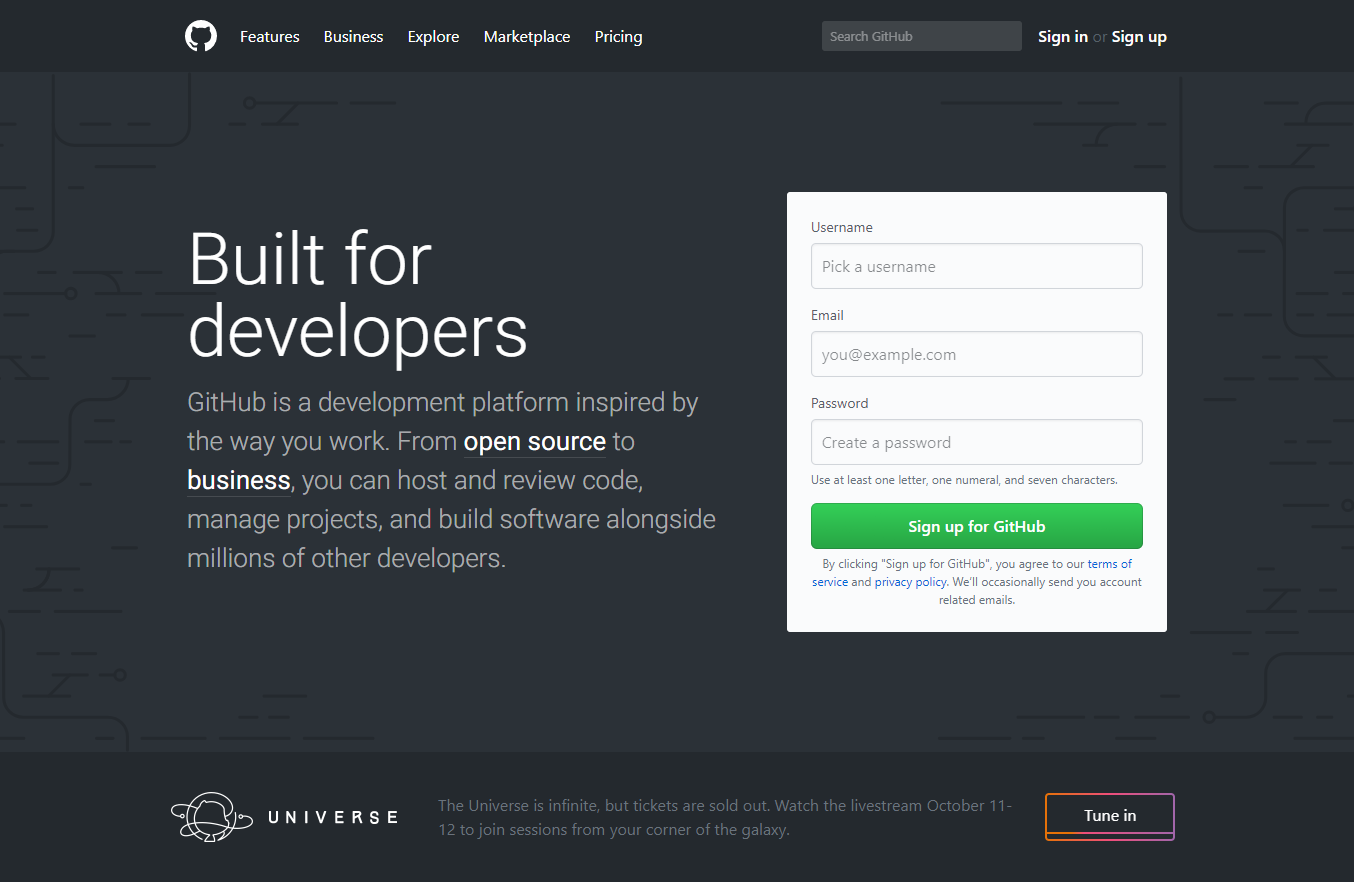
\includegraphics[width=13cm]{img/github.png}
\caption{GitHub}
\end{figure}

\newpage
GitHub Statusは,GitHubにおける関連サービスのステータスを継続的に状況監視しているWebサイトのことである.GitHubの関連サービスが中断した場合は,ここに記録が掲載される.

\begin{figure}[htb]
\centering
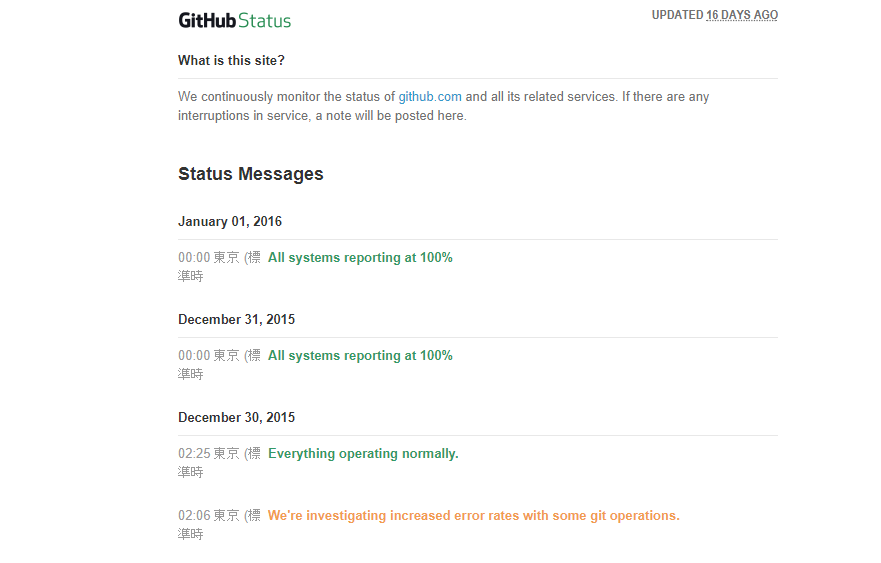
\includegraphics[width=13cm]{img/status.png}
\caption{GitHub Status}
\end{figure}

\newpage

\subsection{Twitter}
Twitter(ツイッター)とは,2006年7月にサービスを開始した140文字以内の短文「ツイート」の投稿を共有するウェブ上の情報サービスである.ほかのユーザーがそれを読んだり,返信をすることでコミュニケーションが生まれるインターネット上のサービスとなっている.従来のソーシャルネットワーキングサービスとは異なる性質を持ったものであり,「ミニブログ」というカテゴリーに分類されている.Twitterにツイートを投稿するにはパソコンや携帯電話,スマートフォンで自身のアカウントを作成,ログインし,画面のボックスに内容を入力し「ツイート」ボタンを押すことで投稿が完了する.ほかのユーザーのつぶやきを追跡することを「フォローする」といい,自分のつぶやきとフォローしたユーザのツイートが同じ画面上に,リアルタイムで表示される.この特徴を利用し,リアルタイムに情報を収集する手段として注目されている\cite{03}.
\begin{figure}[htb]
\centering
\includegraphics[width=13cm]{img/Twitterweb.png}
\caption{Twitter公式}
\end{figure}
\newpage
1つツイートは様々な情報を持っており,主に以下のようなデータを得ることができる\cite{04}.
\begin{table}[htb]
   \caption{ツイートから得られる主なデータ}
  \begin{tabular}{|p{6cm}|p{6cm}|} \hline 
   TweetID & ツイートID \\ \hline
   created\_at  & ツイート作成日.GMT表記   \\ \hline
   User & ツイートを行ったユーザの情報 \\ \hline
   text & ツイート本文 \\ \hline
   source & ツイートを投稿したアプリ \\ \hline
   GeoLocation & ツイートをした緯度経度 \\ \hline
   retweet\_count & リツイートされた数 \\ \hline 
  \end{tabular}
\end{table}

\newpage
Twitterでは,Twitter APIで検索できない期間や数で絞り込むといった高度な検索が利用できる.高度な検索では,検索結果を特定の期間や特定のユーザーなどに絞り込むことができ,探しているツイートも見つけやすくなる.
\begin{figure}[htb]
\centering
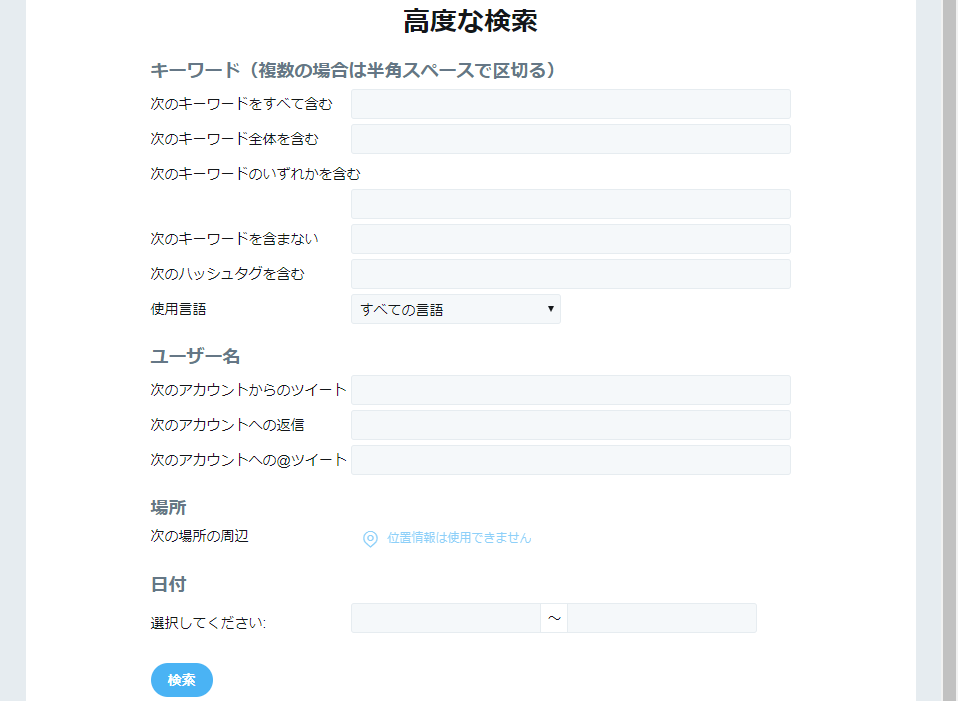
\includegraphics[width=13cm]{img/Twitter.png}
\caption{Twitterの高度な検索}
\end{figure}

また,検索コマンド(演算子)を使用することで,2つ以上の単語検索や完全一致の単語検索などもできる.これらの検索コマンドを一部抜粋し,下記に記した.

\subsubsection{since検索}
「検索したいワード since:年-月-日」と入力すると,検索したいワードを,指定した年月日から現在までに絞り込んで表示させることができる.
\subsubsection{until検索}
「(検索したいワード) until:年-月-日」と入力すると,今度は検索したいワードを,過去から指定した年月日までに絞り込んで表示させることができる.
\subsubsection{from検索}
「from:ユーザーID名」とすると,入力したユーザーがしたツイートのみに絞って検索を行うことができる.
\subsubsection{-検索}
「(検索したいワード) -(検索から除外したい言葉)」のように,半角の「-」を検索したくない言葉の前に付けると,特定の言葉を除外することができる.
\subsubsection{and検索}
2つのワード両方を含むツイートが表示されるように,半角スペースで区切った複数のワードを含む物を検索する.
\subsubsection{OR検索}
複数の言葉の間を「 OR 」と区切ると,少なくとも1つの検索ワードを含むツイートを検索することができる.ORは大文字,ORの両側に半角スペースを入れる必要があり,使用する際は注意が必要である.
\subsubsection{完全一致検索}
“検索ワード”と検索すると,“”内と完全に一致したワードを含むツイートのみが表示される.
\newpage

\section{主な手順}
本研究は以下の2段階で行う.
\begin{enumerate}
 \item Twitterからツイートを収集するためのツールを開発する.
 \item サービスの停止から復旧までに投稿されたGitHubに対するツイート数と,どのくらいの時間で復旧が完了するのかを調べる.
\end{enumerate}

初めに,Twitterで投稿されているGitHubの障害発生に関するツイートをデータとして収集する.TwitterのAPIには,1週間以上前のツイートを検索して取得することができないという制限があるため,本研究のためには使えない\cite{02}.そこで,インターネットブラウザ上のTwitterで使用できる「高度な検索」を利用する(後述).本調査では「キーワード,言語,日時,期間」を指定して検索する.例えば,序論で述べた2016年1月28日に発生したGitHubの障害発生について検索する場合,「GitHub lang:ja since:2016-01-28\_00:00:00\_JST until:2016-01-29\_00:00:00\_JST」となる.検索結果はブラウザを最下部までスクロールすることで古いものが読み込まれていく.これを繰り返すことで,2016年1月28日に投稿された「GitHub」を含む日本語のツイートを全て表示できる.このブラウザを使ったTwitterの検索画面からツイートの本文と時間のみをWebスクレイピングするためのツールを開発し,過去のツイートを取得する.

ブラウザのTwitter検索結果からデータを収集するツールを開発するために2つのプログラムを作成する.1つ目のプログラムでは検索画面を最下部までスクロールする作業とページ全体をHTMLファイルで保存する作業を自動化する.ブラウザのスクロール作業を自動で行う必要があるため,ブラウザの自動操作ができるライブラリである「Selenium WebDriver」を使用し,検索結果をブラウザに全て表示させてからHTMLファイルで保存する.2つ目のプログラムでは,保存したHTMLファイルからツイートの本文と時間のみ抽出するため,Pythonのライブラリであり,HTMLファイルを解析してスクレイピングを行うことのできる「BeautifulSoup4」を使ってデータを抽出する.

データを取得する日を特定するため,GitHubに関連するすべてのサービスを継続的に状況監視している「GitHub Status」の「Status Message」を参照し,2016年で主要なサービスが停止,復旧したとアナウンスされている時間を調べる.その日のツイートを作成したツールを使って検索し,ツイートの時間と本文のみを抽出する.これを各障害の発生日ごとに実行する.これから記載する内容は,\url{https://github.com/ShoIwase/twitter_scraper}にも記載している.



\newpage
\section{研究データの取得}

本研究を進める上での環境構築について解説する.

\subsection{Chocolateyのインストール}
研究で使用するソフトウェアの導入をするため,Chocolateyをインストールする.

\begin{figure}[htb]
\centering
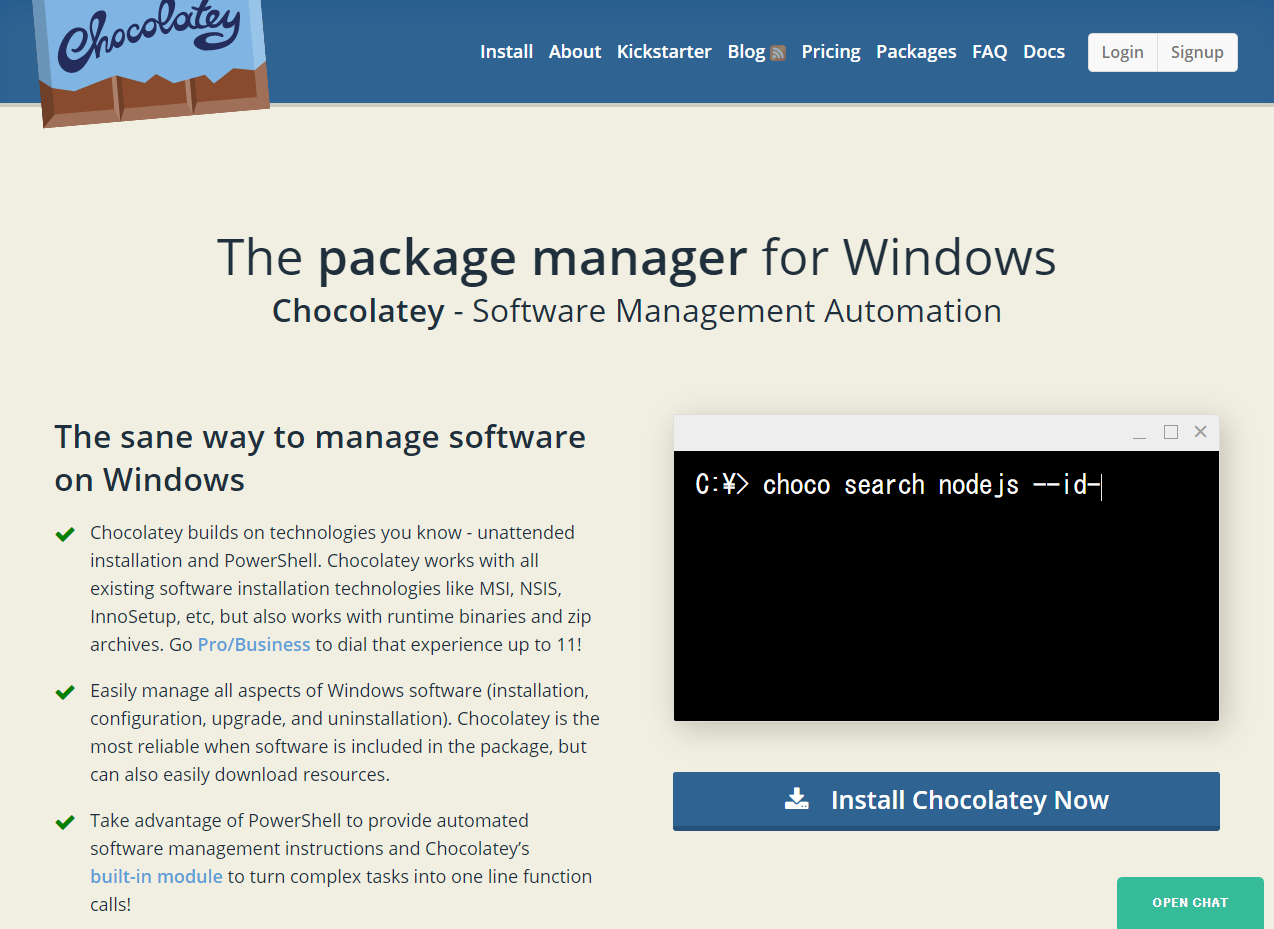
\includegraphics[width=13cm]{img/choco1.png}
\caption{chocoratey公式サイト}
\end{figure}

ChocolateyとはWindows上で動作するソフトウェアをコマンドラインからインストールすることができるパッケージマネージャーである.また,アップグレードやアンインストールと言った管理もできるようになる.

\newpage
WindowsにChocolateyをインストールするためには,管理者権限でコマンドプロンプトを起動し,以下のコマンドを入力するか,公式サイトの「Install with cmd.exe」に載っているテキストをコピーし,コマンドプロンプトに貼り付けて実行すれば良い.


\begin{lstlisting}[breaklines = true, basicstyle=\ttfamily\footnotesize, frame=single]
@"%SystemRoot%\System32\WindowsPowerShell\v1.0\powershell.exe" -NoProfile -InputFormat None -ExecutionPolicy Bypass -Command "iex ((New-Object System.Net.WebClient).DownloadString('https://chocolatey.org/install.ps1'))" && SET "PATH=%PATH%;%ALLUSERSPROFILE%\chocolatey\bin"
\end{lstlisting}

\begin{figure}[htb]
\centering
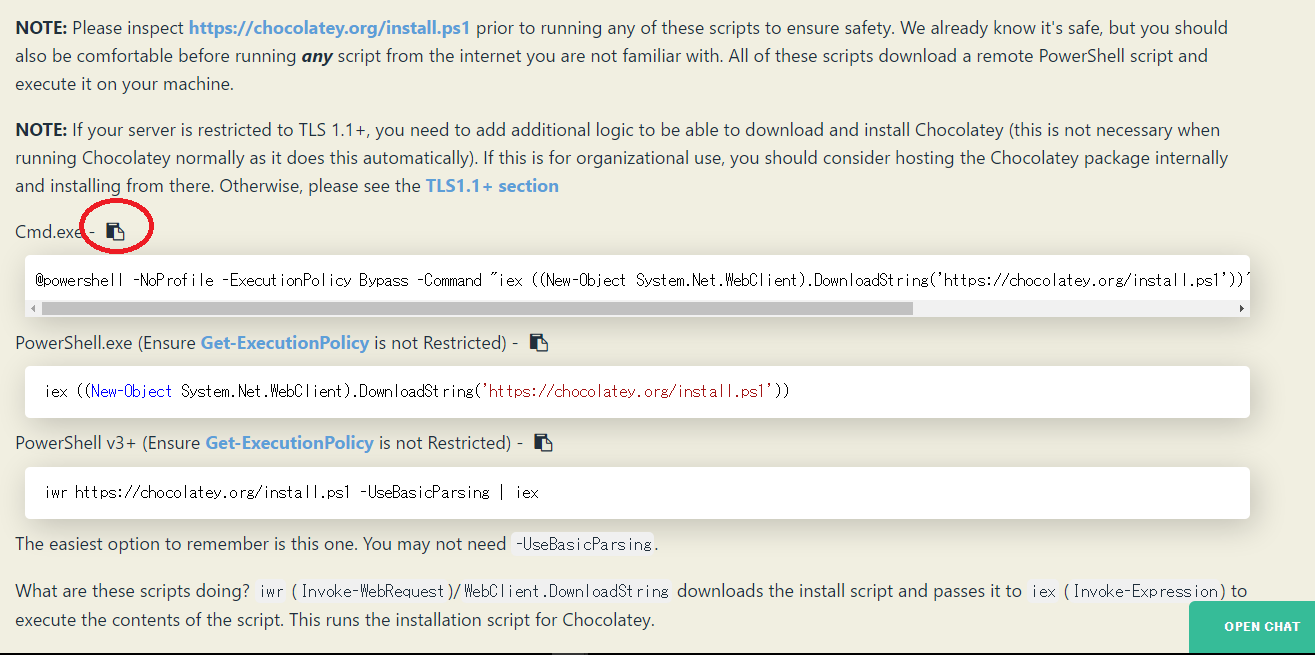
\includegraphics[width=13cm]{img/choco2.png}
\caption{chocorateyのインストールコマンド}
\end{figure}

Chocolateyで使用できるコマンドは次の通りである(cは本来chocoであり,省略されている).
\subsubsection{clist [packageName]}
パッケージ検索をする.引数がなければすべてのパッケージが表示される.
\subsubsection{clist -lo [packageName]}
インストール済みのパッケージ検索をする.引数がなければすべてのインストール済みパッケージが表示される.
\subsubsection{cinst [packageName]}
指定パッケージのインストールをする.
\subsubsection{cuninst [packageName]}
指定パッケージのアンインストールをする.
\subsubsection{cup}
Chocolatey本体のアップデートをする.
\subsubsection{cup [packageName]}
指定パッケージのアップデートをする.
\subsubsection{cup all}
インストール済みのパッケージを全てアップデートをする.


\newpage

Chocolateyをインストール後,環境構築に必要なソフトウェアである「VirtualBox」と「Vagrant」をコマンドプロンプトからインストールする.方法は,コマンドプロンプト(管理者)で公式サイトに掲載されている以下のコマンドを実行すれば良い.

\begin{figure}[htb]
\centering
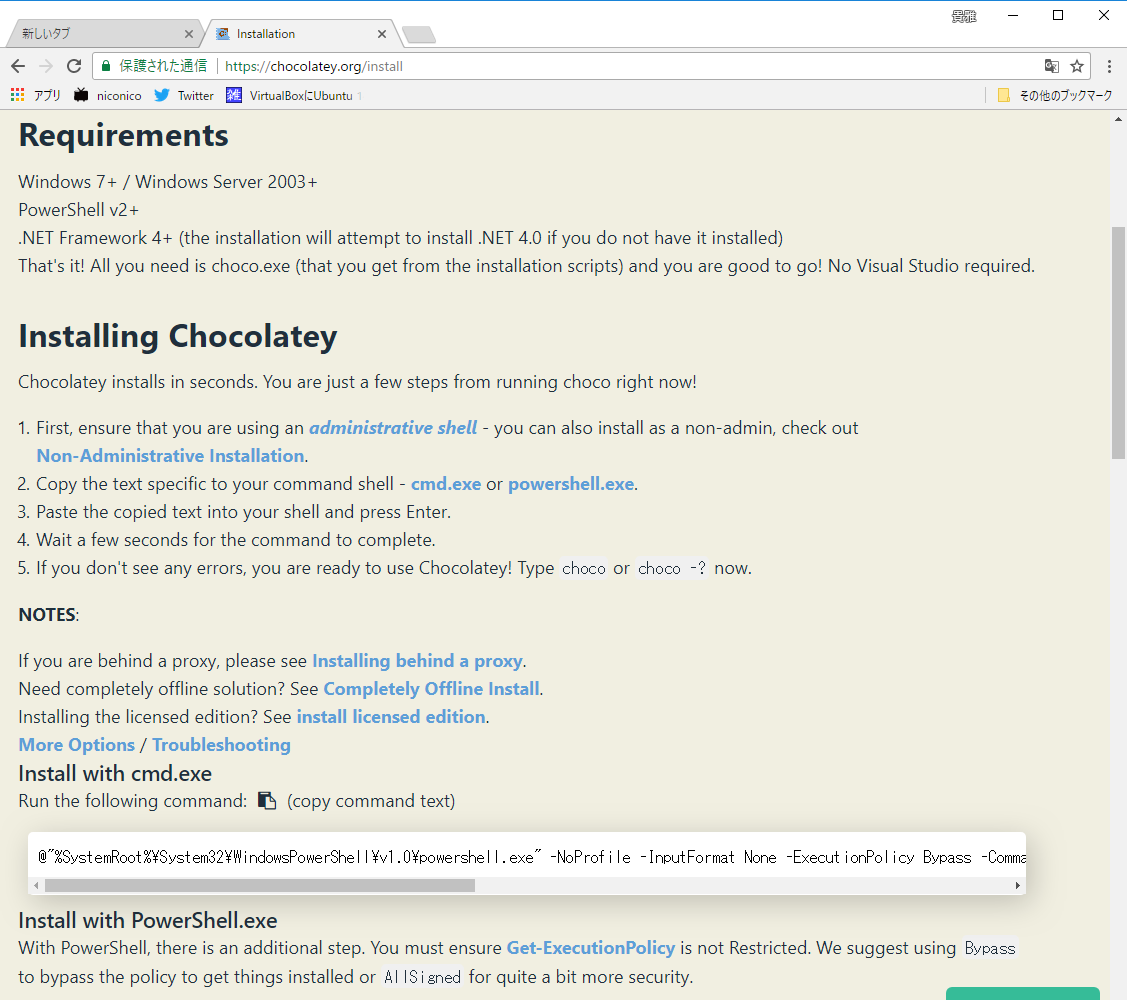
\includegraphics[width=13cm]{img/choco3.png}
\caption{パッケージインストールの実行画面}
\end{figure}

\begin{lstlisting}[basicstyle=\ttfamily\footnotesize, frame=single]
cinst -y virtualbox vagrant
\end{lstlisting}

以上で使用するソフトウェアのインストールは完了である.

\newpage
\subsection{仮想環境の構築}
仮想環境の構築をするため,「VirtualBox」と「Vagrant」をインストールする.
\subsubsection{VirtualBox}
Oracle VM VirtualBoxはOracleが開発,提供するソフトウェアである.使用しているPCに仮想環境を構築してくれるクロスプラットフォーム(Windows,Mac,Linux)対応のフリーソフトである.ホストOS上にゲストOS(これを仮想マシンという)を実装することができる.この解説ではWindows 10をホストOS,Ubuntu 14.04をゲストOSとしている.
\begin{figure}[htb]
\centering
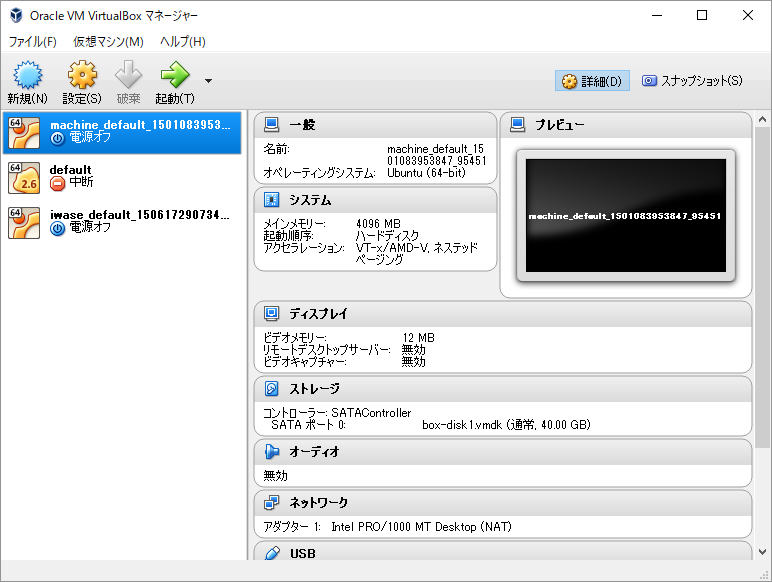
\includegraphics[width=13cm]{img/box.png}
\caption{VirtualBox}
\end{figure}

\newpage
\subsubsection{Vagrant}
Vagrantとは,開発環境の構築と共有を簡単に行うためのツールである.どこでも同じ環境を再現できるように仮想マシン環境を管理する機能が提供されている.Vagrantは,アプリケーションやシステム開発のバックエンドを簡単にパッケージ化し,共有するためのツールである.このパッケージ化された環境を「box」と呼ばれる単位で管理している.

本研究では,矢吹研究室の公式マシンを使用した.このマシンは矢吹研究室のGitHubで公開されており,以下のURLからダウンロードして使用できる.また,公式マシンではUbuntu 16を使用しており,スクリーンショットではUbuntu 14を使用していることがあるが,どちらのOSでも基本的な操作は同じでライブラリやツールは使うことができる.

\begin{verbatim}
https://github.com/yabukilab/machine
\end{verbatim}

ダウンロード方法は,Cドライブにvagrant というディレクトリを作成し,上記のマシンをcloneする.


今後は,このディレクトリで作業を進めていく.

\newpage



\section{Twitter検索結果の取得}
Twitterの高度な検索を用いて研究を行うため,自動的にブラウザを操作する必要がある.そのためにSeleniumを使用する.Seleniumとは,Webブラウザを使ってWebアプリケーションをテストするツールである.この「Webブラウザを使って」というのが非常に大きなポイントであり,人が手でWebブラウザを操作する代わりにSeleniumがWebブラウザを操作してくれる.本研究では,このSeleniumでTwitterの検索結果をスクロールし,全て表示させる.その後,HTMLファイルを出力する.

\subsection{仮想マシンの起動}
仮想マシンを起動するため,コマンドプロンプトを開き以下のコマンドを入力する.
\begin{lstlisting}[basicstyle=\ttfamily\footnotesize, frame=single]
cd /vagrant/i_machine
vagrant up
\end{lstlisting}

仮想マシンの再起動や停止,削除をしたい場合は次のコマンドを使用する.
\begin{itemize}
 \item 仮想マシンを再起動する:\texttt{vagrant reload}
 \item 仮想マシンを停止する:\texttt{vagrant halt}
 \item 仮想マシンを削除する:\texttt{vagrant destroy}
\end{itemize}
\newpage
次に\texttt{vagrant ssh}と入力し,図のようになれば仮想マシンと接続は完了である.
\begin{figure}[htb]
\centering
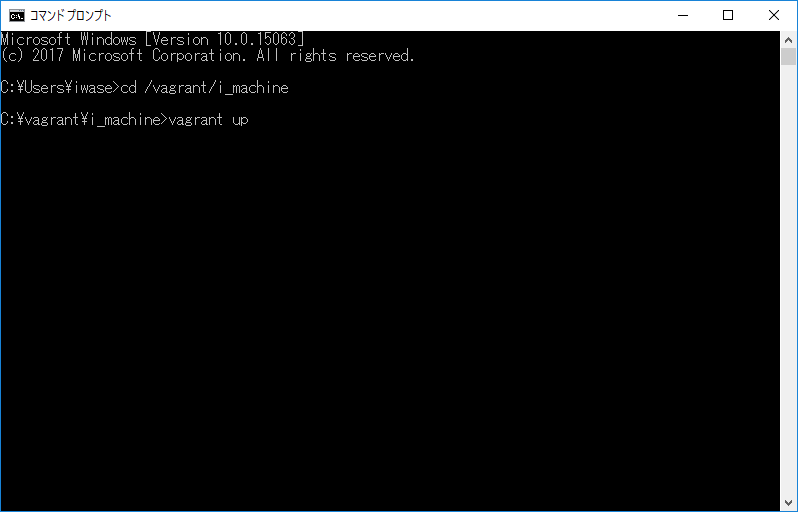
\includegraphics[width=13cm]{img/up.png}
\caption{vagrant up}
\end{figure}

\newpage
\begin{figure}[htb]
\centering
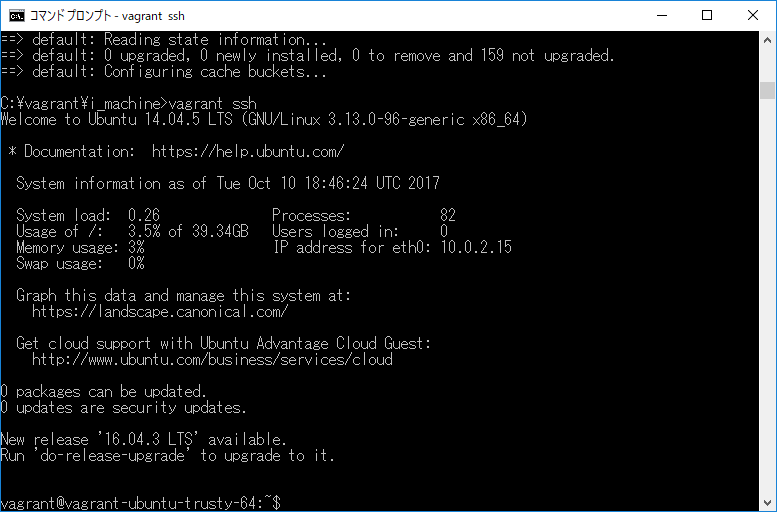
\includegraphics[width=13cm]{img/ssh.png}
\caption{ssh接続}
\end{figure}
切断したい場合はexitと入力する.
\newpage

\subsection{Seleniumのインストール}
Seleniumをインストールするコマンドは次の通りである.
\begin{lstlisting}[basicstyle=\ttfamily\footnotesize, frame=single]
sudo apt-get -y install python-pip
sudo pip install selenium
\end{lstlisting}
\begin{figure}[htb]
\centering
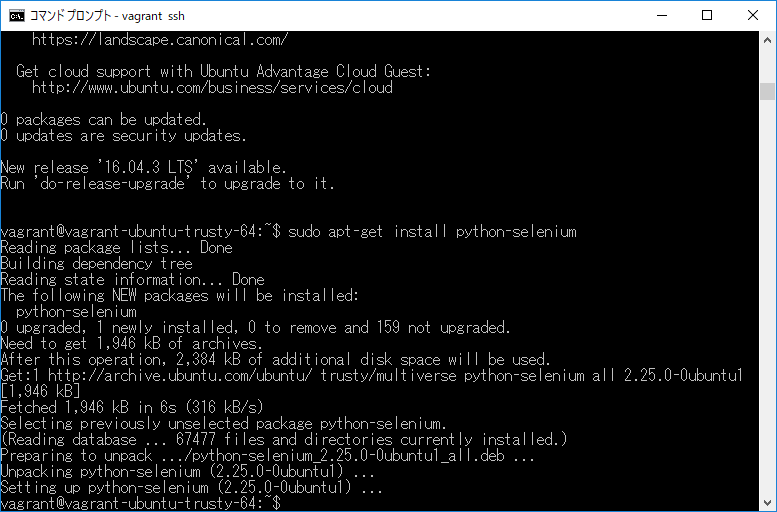
\includegraphics[width=13cm]{img/selenium.png}
\caption{Seleniumのインストール画面}
\end{figure}

\newpage
\subsection{バーチャルモニター(Xvfb)とFirefoxのインストール}
バーチャルモニター(Xvfb)とFirefoxをインストールするため,次のコマンドを入力する.Xvfbとは仮想ディスプレイのことである.Xvfbをインストールすると実際にスクリーンがない状態でも GUI が必要なソフトウェアを使える.FirefoxはWebサイトで検索を行うためのブラウザである.下の2行はブラウザで文字を表示させるために必要なフォントのインストールである.
\begin{lstlisting}[basicstyle=\ttfamily\footnotesize, frame=single]
sudo apt-get -y install firefox xvfb
sudo aptitude install xfonts-100dpi xfonts-75dpi xfonts-scalable 
xfonts-cyrillic
sudo apt-get install fonts-ipafont-gothic fonts-ipafont-mincho
\end{lstlisting}

\begin{figure}[htb]
\centering

\includegraphics[width=13cm]{img/firefox.png}
\caption{XvfbとFirefoxのインストール}
\end{figure}

\newpage
\subsubsection{WebDriverのダウンロード}
\begin{figure}[htb]
\centering
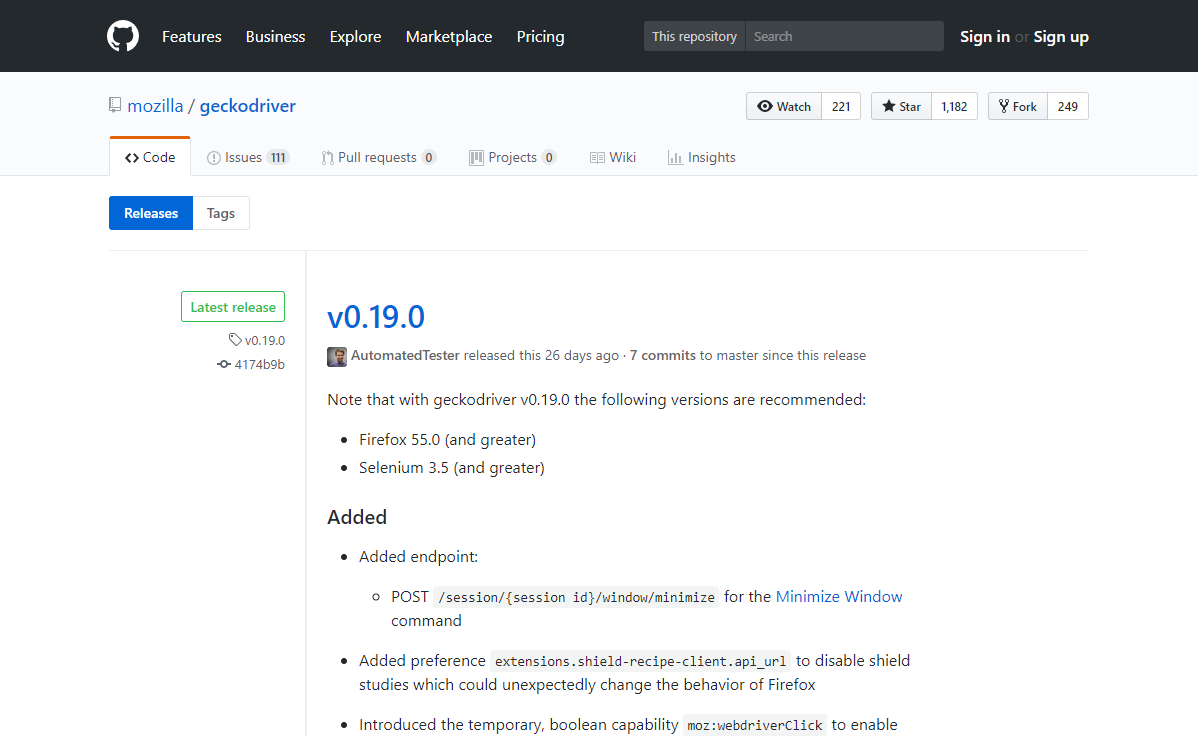
\includegraphics[width=13cm]{img/driver.png}
\caption{geckodriverの配布サイト}
\end{figure}
FirefoxをSeleniumで操作するためには,Firefox用のWebDriverが必要である.Firefox用のWebDriverはhttps://github.com/mozilla/geckodriver/releasesからダウンロードできる.

\newpage
\begin{figure}[htb]
\centering
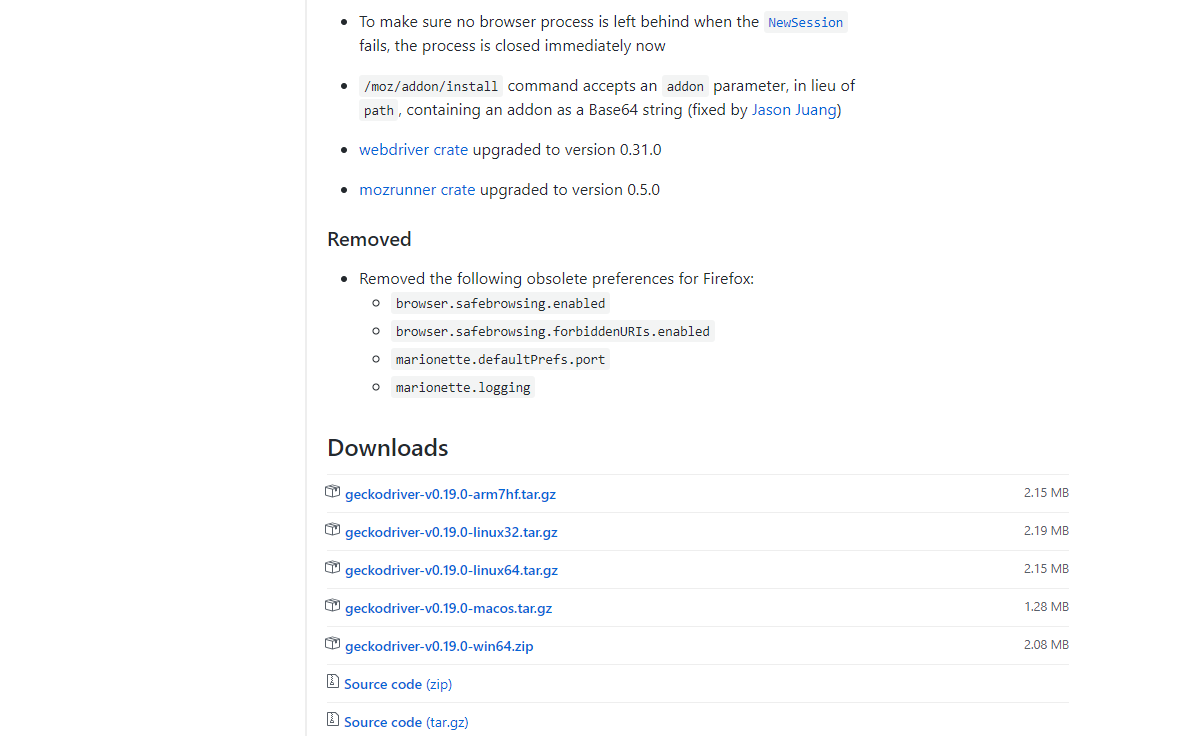
\includegraphics[width=13cm]{img/driver1.png}
\caption{Linux用のgeckodriverを選択}
\end{figure}
使用しているOSは64bitのLinuxのため,\texttt{geckodriver-v0.19.0-linux64.tar.gz}をダウンロードし,解凍する.そして解凍したフォルダの中にあるgeckodriver.exeを作業ディレクトリに配置する.またはPATHが通っているところに置く.
\begin{lstlisting}[basicstyle=\ttfamily\footnotesize, frame=single]
sudo cp ./geckodriver /usr/local/bin
\end{lstlisting}

\newpage

\subsection{プログラムの実行}
Xvfbの起動とディスプレイの設定をするため,次の通りにコマンドを入力する.
\begin{lstlisting}[basicstyle=\ttfamily\footnotesize, frame=single]
sudo Xvfb :99 -ac -screen 0 1024x768x8 &
export DISPLAY=:99
\end{lstlisting}
\begin{figure}[htb]
\centering
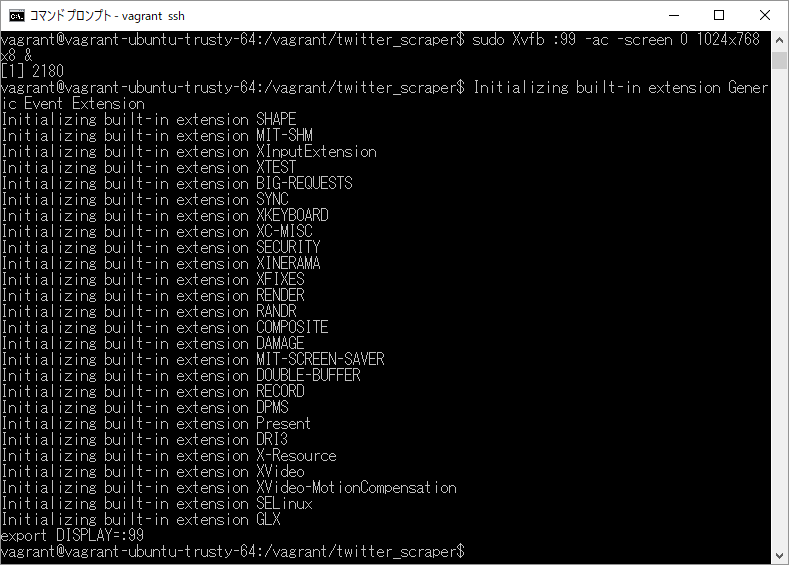
\includegraphics[width=13cm]{img/xvfb.png}
\caption{Xvfbの起動}
\end{figure}

\newpage
実行するプログラム(scroll.py)のソースコードは次の通りである.
\begin{lstlisting}[breaklines = true, basicstyle=\ttfamily\footnotesize, frame=single]
# coding: utf-8
import time
import sys
from urllib import urlencode
from selenium import webdriver

argv = sys.argv
argc = len(argv)
print argv
print argc

url = 'https://twitter.com/search?f=tweets&q=github%20lang%3Aja%20since%3A'+str(argv[1])+'-'+str(argv[2])+'-'+str(argv[3])+'_00%3A00%3A00_JST%20until%3A'+str(argv[1])+'-'+str(argv[4])+'-'+str(argv[5])+'_00%3A00%3A00_JST&src=typd'

print url

# ブラウザ起動
driver = webdriver.Firefox()

# twitter検索結果表示
driver.get(url)

# 一番下までスクロール
lastHeight = driver.execute_script("return document.body.scrollHeight")
while True:
    driver.execute_script("window.scrollTo(0, document.body.scrollHeight);")
    time.sleep(5)
    newHeight = driver.execute_script("return document.body.scrollHeight")
    if newHeight == lastHeight:
        break
    lastHeight = newHeight
    
# HTML出力
data = driver.page_source.encode('utf-8')
print(data)

# 確認のためスクリーンショットを撮る
driver.save_screenshot('result.png')

# 終了
driver.close()

\end{lstlisting}
\newpage
例として以下のようにコマンドを入力し,プログラムを実行すると2016年4月6日のツイートが検索され,0406.htmlというHTMLファイルが実行したディレクトリに出力される.
\begin{lstlisting}[basicstyle=\ttfamily\footnotesize, frame=single]
python scroll.py 2016 04 06 04 07 > 0406.html
\end{lstlisting}

\begin{figure}[htb]
\centering

\includegraphics[width=13cm]{img/0406.png}
\caption{プログラムの実行}
\end{figure}
\newpage
次の画像が実際に出力されたHTMLファイルの中身である.

\begin{figure}[htb]
\centering
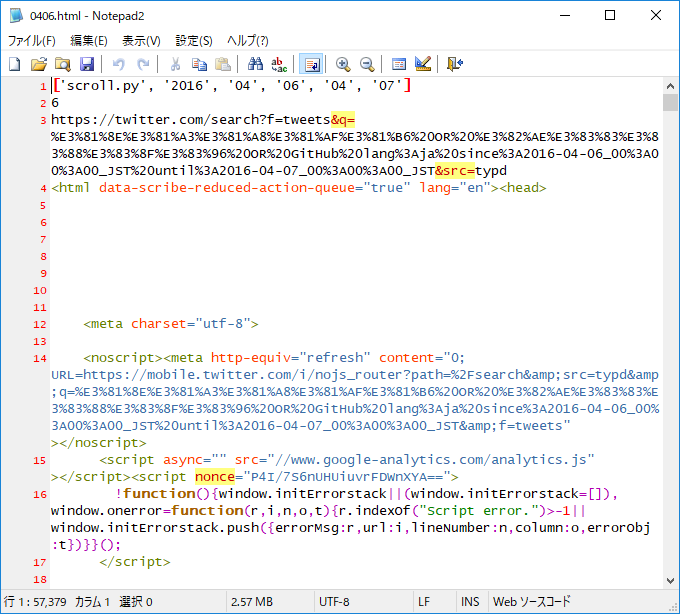
\includegraphics[width=13cm]{img/html.png}
\caption{出力されたHTMLファイル}
\end{figure}

GitHub Statusを参照にGitHubがサービス停止したと報告されている日を調べ,その日ごとにこの手順を繰り返し,HTMLファイルを収集する.

\newpage
\section{データの抽出}
保存したHTMLファイルから特定のデータを抽出・整形するため,Webスクレイピングをする.Webスクレイピングを行うことで,Webページを対象として,あたかもAPIを利用しているかのようにデータを効率的に取得・収集することが可能になる.
\subsection{BeautifulSoup4のインストール}
「BeautifulSoup4」とはWebスクレイピングで使われるPythonのライブラリである.特徴はとしては,HTMLやXMLの構造を解析して,特定の要素を指定しやすい形に加工できることや,XpathやCSSセレクタを使った要素の抽出を行うことができることが挙げられる.

BeautifulSoup4のインストールコマンドは以下の通りである.
\begin{lstlisting}[basicstyle=\ttfamily\footnotesize, frame=single]
sudo pip install BeautifulSoup4
\end{lstlisting}
以上でスクレイピングをする準備が整った.

\newpage
\subsection{プログラムの実行}
スクレイピングをするプログラム(scrape.py)のソースコードは次の通りである.
\begin{lstlisting}[breaklines = true, basicstyle=\ttfamily\footnotesize, frame=single]
# coding: utf-8
import sys
from bs4 import BeautifulSoup
from datetime import datetime

soup = BeautifulSoup(sys.stdin,"html.parser")
tweets = soup.findAll('li',{"class":'js-stream-item'})

for tweet in tweets:
    if tweet.find('p',{"class":'tweet-text'}):
        tweet_time = datetime.fromtimestamp(int(tweet.find('span', '_timestamp')['data-time']))
        tweet_text = tweet.find('p',{"class":'tweet-text'}).text.encode('utf8').replace("\n", "").replace(",", "")
        
        print tweet_time,
        print ',',
        print tweet_text
    else:
        continue
\end{lstlisting}

上記のプログラムを実行し,保存したHTMLからツイートの時間と本文をスクレイピングするためには次のコマンドを入力する.
\begin{lstlisting}[basicstyle=\ttfamily\footnotesize, frame=single]
python scrape.py < 0406.html
\end{lstlisting}

\newpage
テキストファイルに出力する場合は次のコマンドを入力する.
\begin{lstlisting}[basicstyle=\ttfamily\footnotesize, frame=single]
python scrape_.py < 0406.html > 0406.txt
\end{lstlisting}


\begin{figure}[htb]
\centering
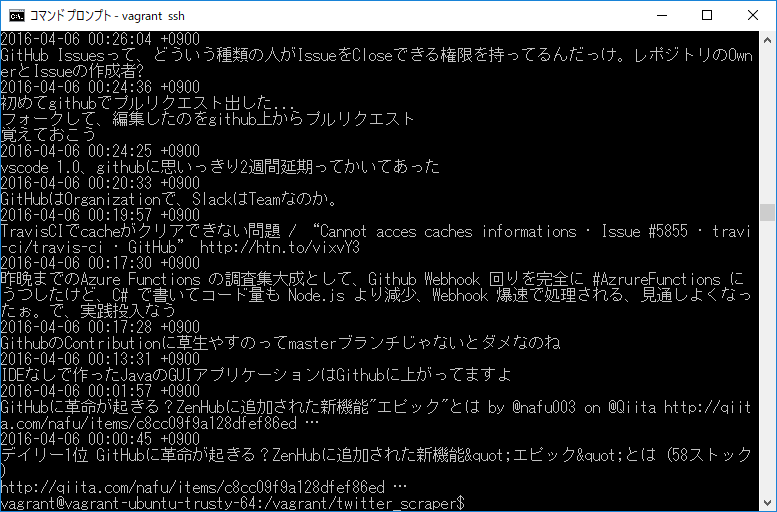
\includegraphics[width=13cm]{img/scraping.png}
\caption{スクレイピング結果}
\end{figure}

この作業をHTMLファイルごとに行う.

\newpage
\subsubsection{シェルスクリプトの使用}
HTMLファイルの数が増え,スクレイピングの処理回数が手間になる場合は,シェルスクリプトを使用する.シェルスクリプトを使用すると,実行ファイルのディレクトリに存在するHTMLファイル全てから上記のスクレイピング一括で実行することができる.ホストで作成したシェルスクリプトを仮想環境で実行するためには,Line EndingsをUnixで保存する必要がある.そのスクリプトファイル(scraping.sh)のソースコードを以下に記す.
\begin{lstlisting}[basicstyle=\ttfamily\footnotesize, frame=single]
#!/usr/bin/env bash
file=*.html
for file in ${file}
do
  python scrape.py < ${file} > ${file%.*}.txt
done
\end{lstlisting}

\newpage
スクリプトを実行するコマンドは以下の通り.
\begin{lstlisting}[basicstyle=\ttfamily\footnotesize, frame=single]
sh scraping.sh
\end{lstlisting}
\begin{figure}[htb]
\centering
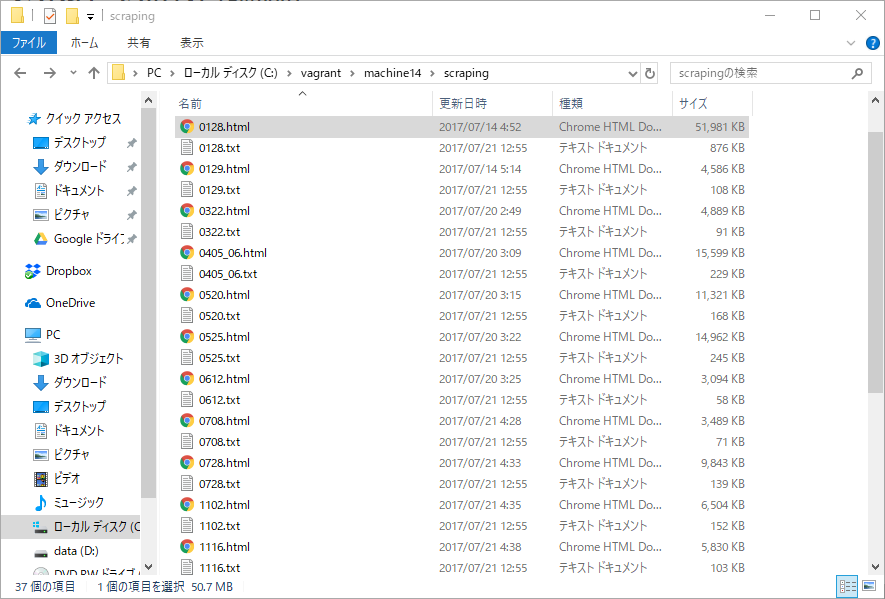
\includegraphics[width=13cm]{img/shell.png}
\caption{シェルスクリプト実行後のフォルダ}
\end{figure}
以上でデータの収集は完了である.

\chapter{結果}
GitHub StatusのStatus Messageを参照に調べたところ,2016年のGitHubにおけるサービス停止回数は14回であった.本研究では,そのうちの13回分を調査する.残りの1回は,同時期にTwitterにも障害が発生していたため,本研究の調査対象とはしない.

13回分の各障害のサービス停止から復旧までの間隔を分単位でグラフにしたものが図\ref{時間}である.
\begin{figure}[htb]
\centering
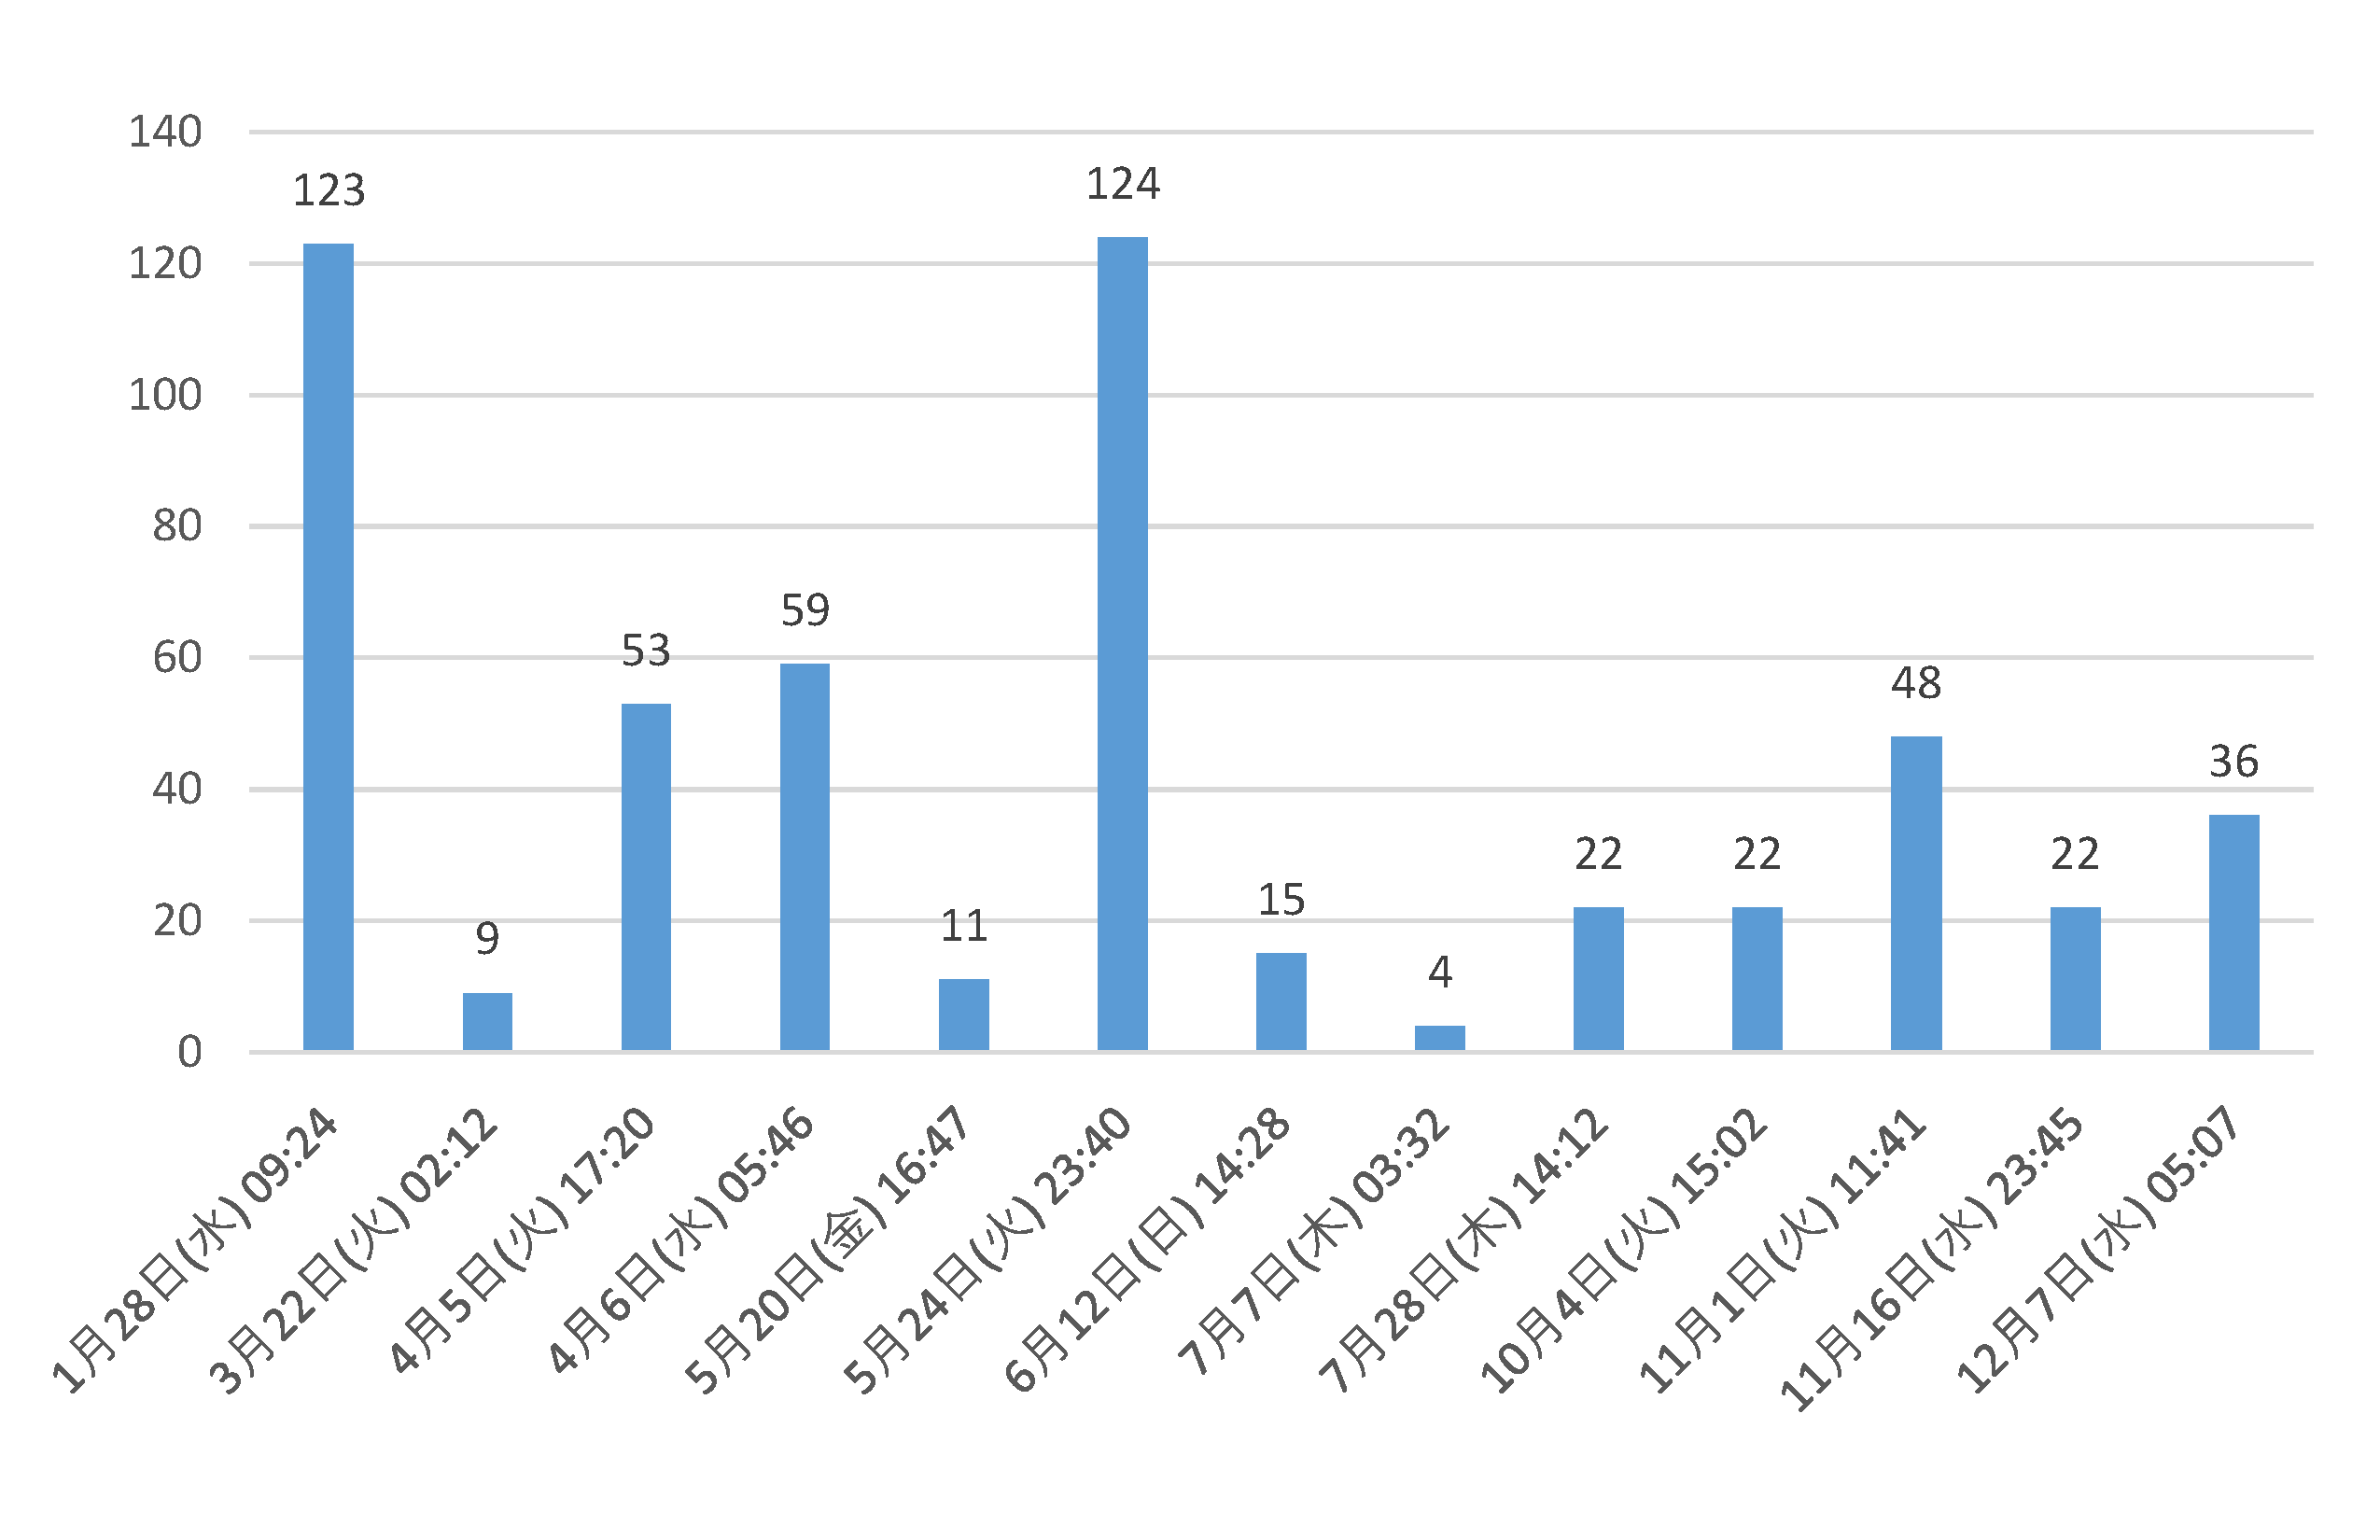
\includegraphics[width=13cm]{img/graph1.pdf}
\caption{サービス停止から復旧までの間隔}\label{時間}
\end{figure}




\newpage
各障害のサービス停止中に投稿されたツイート数をグラフにしたものが図\ref{ツイート数}である.
\begin{figure}[htb]
\centering
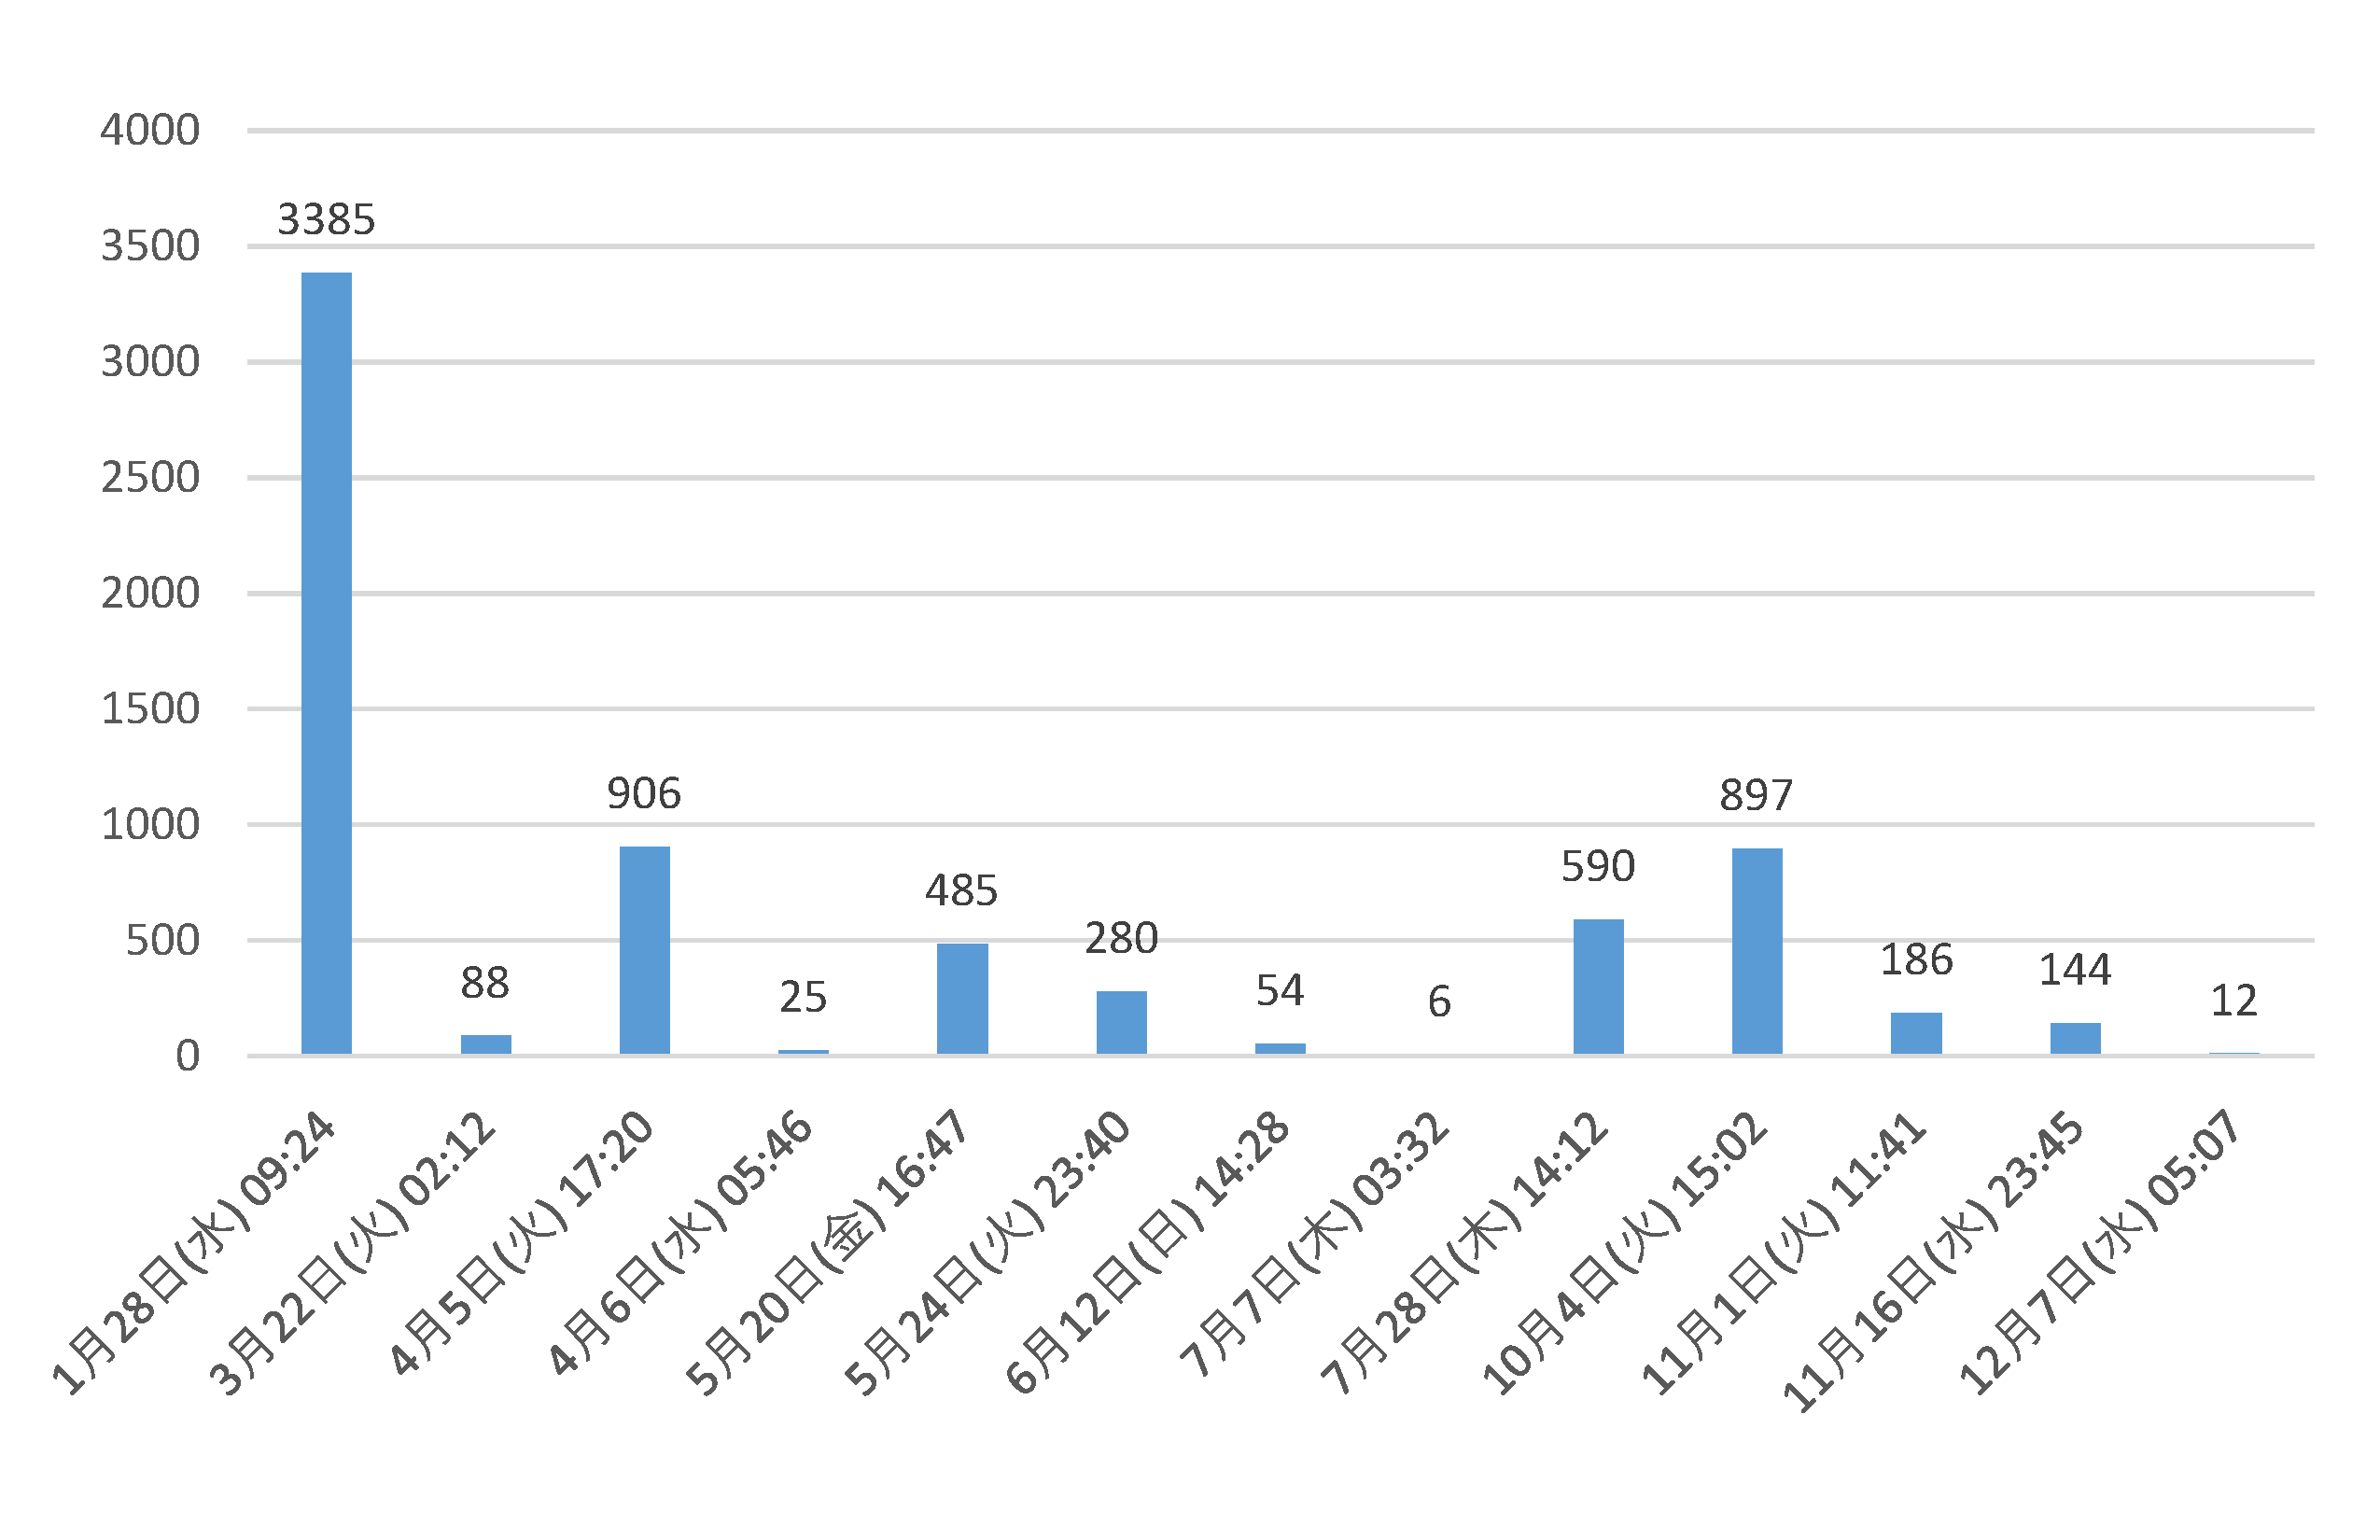
\includegraphics[width=13cm]{img/graph2.pdf}
\caption{サービス停止中に投稿されたツイートの数}\label{ツイート数}
\end{figure}
\newpage
縦軸をツイート数,横軸を停止時間としてサービス停止時間に対するツイート数を見るための散布図を作成した.それが図\ref{散布図}である.
\begin{figure}[htb]
\centering
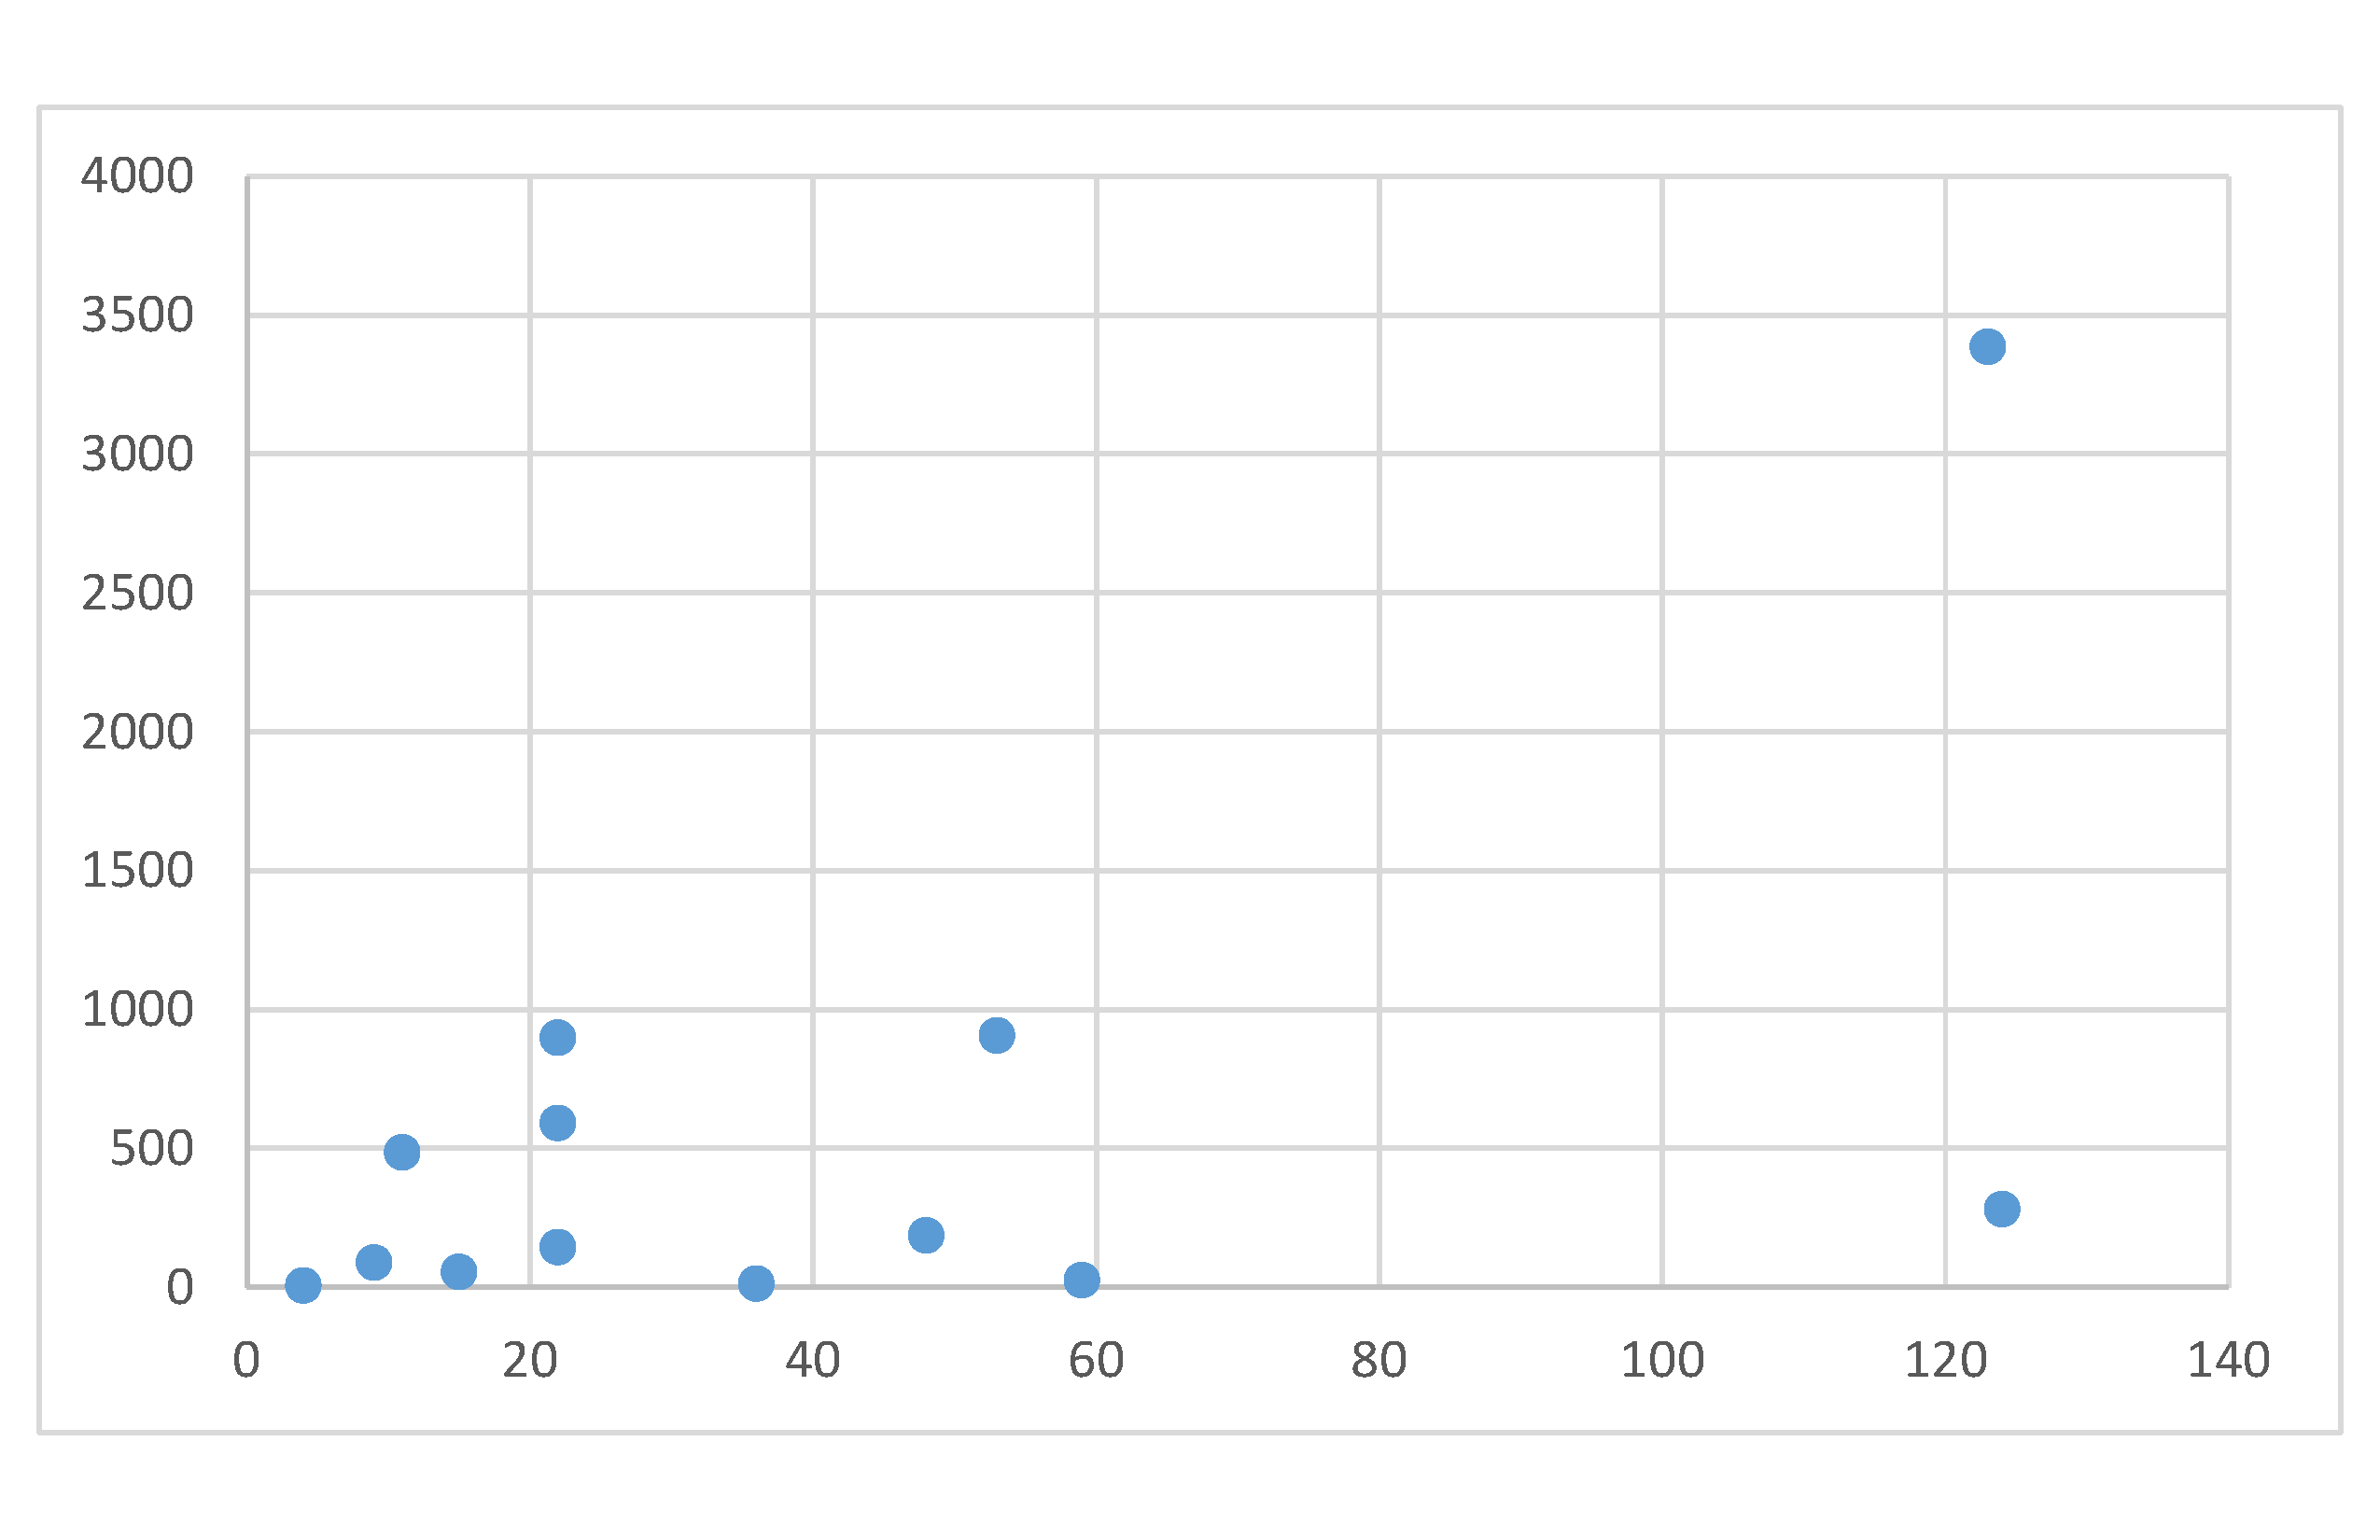
\includegraphics[width=13cm]{img/sample.pdf}
\caption{サービス停止時間に対するツイート数}\label{散布図}
\end{figure}

\newpage
取得したファイルの一つである,2016年5月20日のサービス停止前後のデータを例として記載する.この日はサービス停止時間が11分間で485ツイートという結果だった.
\\
\begin{verbatim}
2016-05-20 17:58:46 , 46件のコメント http://b.hatena.ne.jp/entry/www.
publickey1.jp/blog/16/github7.html#tw?u=magamin … “[速報]GitHub、月額7ドルでプライベートリポジトリを無制限に作成可能に。新料金プランを発表 - Publickey” http://htn.to/KWTp36 
2016-05-20 17:58:29 , Githubを厳しい第三者の目で見る
2016-05-20 17:57:10 , githubおちてるのか
2016-05-20 17:56:45 , そうか…streakなくなったのか…一応続けてたのですごい残念。 / 他31コメント http://b.hatena.ne.jp/entry/s/github.com/blog/2173-
more-contributions-on-your-profile#tw?u=igrep … “More contributions 
on your profile · GitHub” http://htn.to/4swpWoPL 
2016-05-20 17:56:34 , またGithub落ちたんかい。
2016-05-20 17:56:15 , GitHubで仕事用アカウントと個人用アカウントを分けているひと、いまのところ25\%くらいか。もそれなりにいるのでちゃんと配慮しよう…。  https://twitter.com/__gfx__/status/733574502848692225 …
2016-05-20 17:56:03 , githubがトレンド入りしてる。
2016-05-20 17:55:54 , 個人的には「GitHubやってる?」よりも「jsdo.itやってる?」を流行らせたい
2016-05-20 17:55:42 , GitHubなにかと思ったら落ちてるのか…
2016-05-20 17:55:23 , GitHub multiple account 設定 - Qiita github の複数アカウント作成      github での複数アカウントの登録をしたときのメモです。        新しいアカウント用の ... http://bit.ly/1XE7o2r 
2016-05-20 17:55:20 , GitHubがダウンしてトレンド入りするくらいGitHub浸透してるんやな
2016-05-20 17:55:09 , GitHubトレンド入りしてる珍しいと思ったら落ちてたのね
2016-05-20 17:54:50 , GitHubとTwitter死んだら,slackが後者の代替品になるんだろうな
2016-05-20 17:54:19 , GitHub祭りに乗り遅れた…みんなオクトキャット(#Octocat )は知ってる?[2月は猫]ネコとタコのキャラクター?「#GitHub 」オクトキャットのゆるカワグッズまとめ - otacco[おたっこ] https://otacco.com/articles/915 
2016-05-20 17:53:51 , github落ちてるらしいっすよ
2016-05-20 17:53:02 , GitHub落ちてトレンド入りしてるw
2016-05-20 17:52:59 , そんなものは戦車道につかった。てか君GitHubやってる?
2016-05-20 17:52:49 , GitHub先生落ちてたのかぁ・・・以前だと帰る時間が遅くなるパターンだ
2016-05-20 17:52:40 , Githubってタコネコさんのことだよ
2016-05-20 17:52:30 , Githubトレンドにあるのは落ちてたのかww金曜日のこの時間辺りに落ちるってことは社畜の皆さんに休めという天からのお達しであろう( ˘ω˘ ) .。oO(なお、復旧した模様)
2016-05-20 17:52:26 , GitHubが落ちてツイッターのトレンドの上位にくるってのがもう草落ち着いてビールでも飲もうや???「おう冷えてるか〜?」???「バッチェ冷えてますよ〜(開発現場)」
2016-05-20 17:52:20 , Githubがトレンドにあるのは落ちてる証拠
2016-05-20 17:51:52 , Gitの話したらGithubのリストに叩きこむの辞めろ
2016-05-20 17:51:47 , また Github 落ちたのか。。
2016-05-20 17:50:45 , 普段は可用性の確保ができてないシステムに厳しいのにGithubが落ちたらビールタイムに突入するなど
2016-05-20 17:50:40 , github落ちたからもう帰りますと言いたい(普通にbacklogのリポジトリで運用しているので帰れない)
2016-05-20 17:50:21 , github落ちは社畜の休憩
2016-05-20 17:49:03 , GitHubトレンド入りに驚く
2016-05-20 17:49:01 , GitHub落ちてトレンド入りしたのか
2016-05-20 17:48:36 , 弊社エンジニア「GitHubが落ちても仕事自体は減らないでしょ??クレジットカードみたいなものでしょ???」
2016-05-20 17:48:29 , gitであってgithubではない
2016-05-20 17:48:24 , GitHub使ってるのか…JSなのに… 
https://twitter.com/milkchan_web/status/733578028656136192 …
2016-05-20 17:47:17 , Github落ちてたってまじ?
2016-05-20 17:47:14 , Githubおちてたとか笑えない
2016-05-20 17:47:05 , これは、あれか。「君LINEやってる?」の代わりに「君GitHubやってる?」が流行るフラグか
2016-05-20 17:46:16 , 今気付いた。トレンドにGitHubの文字がある
2016-05-20 17:45:57 , github先生調子悪かったのか。
2016-05-20 17:45:50 , 戻ったみたいですね。"GitHub down" 
https://status.github.com/graphs/past_day 
2016-05-20 17:45:39 , github復活したから就業継続っす
2016-05-20 17:45:28 , githubが死ぬことで社畜が救われる?
2016-05-20 17:45:05 , お。github復活したか。
2016-05-20 17:44:35 , GitHubかトレンドに入ってる(・・?
2016-05-20 17:43:04 , GitHubアクセスしたらオラついたユニコーン出てきてきめぇ
2016-05-20 17:42:27 , またGitHubか
2016-05-20 17:41:10 , GitHub落ちてんの?んじゃ今日は閉店じゃー三╰( 'ω’)╯
2016-05-20 17:40:56 , Githubがトレンドに入っててワロタ pic.twitter.com/jUyazhidnt
2016-05-20 17:40:05 , GitHub落ちてる
2016-05-20 17:39:58 , なぜトレンドにGitHubが
2016-05-20 17:39:41 , あー、ついにGithubがpersonal planでprivateリポジトリ無制限になった。http://buff.ly/22hSNdv 
2016-05-20 17:39:37 , github落ちた祭りか
2016-05-20 17:39:27 , GitHub「お前らのせいでもう手遅れな」ってどうよ?
2016-05-20 17:38:24 , なんかGitHub落ちた後UI変わったんじゃないかな???(clone or copyとか)
2016-05-20 17:38:03 , GitHub落ちたん?
2016-05-20 17:37:16 , Github Pages の RSS 便利ですね
2016-05-20 17:36:51 , github 落ちた祭り乗り遅れた
2016-05-20 17:36:36 , 一方、我が社ではGithubはWebフィルタの対象でアクセスができなかった(白目)
2016-05-20 17:36:34 , GitHub落ちたから飲みに行こう みたいなつぶやき溢れてる
2016-05-20 17:35:59 , GitHubがトレンドに入るということは落ちたのか。
2016-05-20 17:35:07 , 「GitHubのサイトからのダウンロード方法」
 http://okwave.jp/qa/q8783494.html?tw=trend … 
 monacaというサイトでiOS用のアプリ作成を行っています。... #GitHub
2016-05-20 17:34:29 , Githubのsyntax highlight、盛大に誤爆していて楽しい。https://github.com/yumetodo/boost_asio_ssl_file_dl_test/blob/master/
boost_asio_ssl_file_dl_test/Source.cpp#L144 …
2016-05-20 17:34:22 , #GitHub、30分ほど前にプライマリーデータベースを修復して既に正常運行に戻ってます。https://twitter.com/githubstatus/status/733568749907771393 …
2016-05-20 17:34:18 , Githubがトレンド入りしたらそれはIT界隈で地震が起きているっての爆笑した
2016-05-20 17:34:07 , Githubがトレンドに...!
2016-05-20 17:34:00 , GitHubって落ちる度にトレンドに入ってるよね
2016-05-20 17:33:53 , GitHubトレンド入りしてる
2016-05-20 17:33:13 , トレンドにGitHub(´・ω・`)
2016-05-20 17:33:07 , ?GitHub落ちたの? (トレンドに出てるのを見て真っ先に思った)
2016-05-20 17:32:46 , GitHubが落ちたくらいじゃ仕事は滞らない。なぜなら弊社ではGitHubを使用していないから(涙)
2016-05-20 17:31:56 , Githubが落ちて業務ができないからTwitterをする人たちからTwitterを奪うなんてひどいことは考えてはいけない
2016-05-20 17:31:52 , GitHub、時々タイムラインはOrganization毎に別々に出してほしいと思うことがある。
2016-05-20 17:31:26 , (´ω`) 。oO(Twitterトレンドが #GitHub のステータス確認機能と化している件。)
2016-05-20 17:31:14 , CodeTreeとかWaffle.ioみたいなGitHubカンバン化サービスを使っていると、GitHubが落ちてもIssueの内容は確認できて便利
2016-05-20 17:31:02 , githubの草の天ぷら
2016-05-20 17:30:48 , 授業でGitHub使って、その後友人がGitHubについてツイートした後にGitHubがトレンド入りするというタイムリーさ
2016-05-20 17:30:42 , GitHubのアカウント、個人用と会社用でわけないのが普通だとおもっていたんだけど、どうもそれは一般的とはいえないんじゃないかという気がしてきたので…。 https://twitter.com/__gfx__/status/733574502848692225 …
2016-05-20 17:30:33 , 見たこと無いんだけどGitHub落ちてるのでリリースやメンテナンスが伸びますって事例はあったんだろうか
2016-05-20 17:30:25 , GitHubおちたのか
2016-05-20 17:30:00 , 日本の現在のトレンド一覧#もう付き合っちゃえよーという二人GitHub#これ見た人は食べたい和菓子をあげる#あなたの喘ぎ声診断第三者#Twitter禁断症状#心汚れ度キンプリ4DXスタージュエル2500個ハァァァァーーー無料10連
2016-05-20 17:29:37 , トレンドに入ってたら落ちてることがわかるGitHub
2016-05-20 17:29:05 , トレンドにGitHubが出るたびに『皆様、お疲れさまでございます』と感じてしまうのは何故なのでしょう…
2016-05-20 17:28:54 , githubも月イチで落ちてる感じがするんだよなぁ
2016-05-20 17:28:47 , Github死んでたの?俺普通にpush出来てたが……?
2016-05-20 17:28:25 , GitHubがtwitterのトレンドワードに入っててワロタ。落ちてたら皆とりあえずtweetするのか
2016-05-20 17:28:08 , github復活したせいで仕事できる……つらい……
2016-05-20 17:27:59 , GitHubがトレンドに入ってるw
2016-05-20 17:27:01 , とある学者の報告によると、GitHubがダウンしてからの数時間、世界中で経済消費が爆発的に上昇するという。 (資料提供: 民明書房)
2016-05-20 17:26:59 , github自体のソースが公開されたとしても、運用ノウハウと実績と信頼性まで付いてくるわけでもないので
2016-05-20 17:26:33 , githubにSchoolIdolFestival投げたけど、なんか今障害でもあったん?
2016-05-20 17:26:32 , Github関係ないけど帰るか。
2016-05-20 17:26:05 , GitHubで仕事用アカウントと個人用アカウントを分けているのかどうか知りたい!!
2016-05-20 17:24:36 , githubしんだの
2016-05-20 17:24:27 , GitHub落ちただと
2016-05-20 17:24:17 , githubダウンしてたのか
2016-05-20 17:23:26 , github、自分から見える草はプライベートレポジトリも含まれてる気がするけど含まない草が見たい。
2016-05-20 17:22:52 , GitHub本体がFLOSS化してたらGitHub Inc.が成り立つのかってのはちょっと興味深いよね、今以上に素のGitLab建てただけのGitホスティングサービスがGitHubに置き換わったものが乱立しそうでどこに商機があるのか
2016-05-20 17:22:19 , トレンドにGitHubあるけどなしたん?
2016-05-20 17:22:13 , ん?またGitHub逝ったの?
2016-05-20 17:22:09 , github落ちてたのか。bitbucketの私に死角はない。
2016-05-20 17:22:00 , 他の仕事やっていた間に、Github復旧してた。
2016-05-20 17:20:18 , Githubが不調で、自分の体調も良くないので、仕事切り上げたいけど、うちそもそもGitlabだ。
2016-05-20 17:20:17 , github復活したから帰ります←
2016-05-20 17:20:15 , 来年あたりからはGitHub使いたい勢です
2016-05-20 17:19:49 , GitHubが落ちていたようだが,GitLabなので問題はなかった
2016-05-20 17:19:35 , githubトレンドってどしたんや
2016-05-20 17:19:17 , GitHubがPornhubに見えた
2016-05-20 17:19:10 , GitHub死亡と聞いて
2016-05-20 17:18:52 , GitHub落ちてたらしいけど、7ドルで無制限になったらしい。しらんかった。 >> GitHubが料金体系改定、プライベートリポジトリの作成が無制限に http://news.mynavi.jp/news/2016/05/12/017/ …
2016-05-20 17:18:34 , GitHubはいいぞ
2016-05-20 17:18:07 , あれ、今回は影響なかったけどまたGitHub落ちてたの?[ #PluCial http://goo.gl/gbcmRM  ]
2016-05-20 17:18:06 , そしてGoogleの検索候補にGitよりもGitHubの方が先に出てきたんだけど
2016-05-20 17:17:45 , なぜGitHubがトレンドに?って思ったら落ちてたのか。
2016-05-20 17:17:44 , GitHubがトレンドにあがってるけど、また落ちたの?
2016-05-20 17:17:41 , Githubがトレンドに
2016-05-20 17:17:20 , GitHubって開発者以外でも有名なの?
2016-05-20 17:17:08 , 彼氏が GitHub enterprise 使ってた...別れたい...
2016-05-20 17:16:53 , サーバーが落ちるたびにトレンドに上がるGitHubちゃんの影響力すごいね。svnのファンになります。
2016-05-20 17:16:41 , Githubトレンド入りしててワロ
2016-05-20 17:16:23 , githubしんだ途端みんな帰ろうとしててワロタw
2016-05-20 17:15:48 , githubトレンド入りしてるとなんかこう、察するよね(´・ω・`)
2016-05-20 17:15:12 , まーたGitHubが落ちたのか
2016-05-20 17:15:12 , githubが落ちると社内チャットにユニコーンがあふれる pic.twitter.com/YVlezrEQG4
2016-05-20 17:14:12 , githubが死んだと聞いて(遅い
2016-05-20 17:13:55 , やっぱり数分間だけエラー発生してたんだね。Status画面では若干のラグがあることを理解しやした。/GitHub System Statushttps://status.
github.com/ 
2016-05-20 17:13:52 , しってるよGitHubがトレンドにある時は落ちてる時なんでしょ pic.twitter.com/EpU5abujRX
2016-05-20 17:13:18 , オフィスで仮眠取ってるうちにGitHubが落ちて復活してたぽいので徳のなせる技といった感じですね
2016-05-20 17:13:15 , 会社によってはむしろGitHubより落ちて帰りやすい…?
2016-05-20 17:12:33 , GitHubが落ちたときに「Github」とか書いたやつはリムれ!
2016-05-20 17:12:13 , あれ、github落ちてたのか
2016-05-20 17:12:05 , Githubが戻ってもやることがないのが社内ニートの特権
2016-05-20 17:12:03 , Githubが落ちた瞬間に、エンジニア達が卓球し始めた。そんな職場です。
2016-05-20 17:11:52 , github が落ちた時のための git daemon の使い方とか Qiita に書くチャンスですよ
2016-05-20 17:11:45 , 「GitHubが落ちたようだが、既に飲んでいるので関係ない」という発言がTLに散見されるのは良いことだと思った。#華金
2016-05-20 17:11:44 , もうgithub復旧したっぽい。早いな。
2016-05-20 17:11:32 , さっきまで数分間、GitHubが500エラーとかでつながらなくなってたのよ。そんなとき、ブラウザにはシュッとしたユニコーンが現れるのさ (キリッ
2016-05-20 17:11:25 , github「休んで良いというサインを出したな、あれは嘘だ」
2016-05-20 17:11:11 , この時間に出社するのが悪い Githubつぶしていけ
2016-05-20 17:11:09 , github死んでるの?
2016-05-20 17:10:54 , github復活したので作業再開
2016-05-20 17:10:51 , GitHubとか何も関係ないんだけど帰りたい
2016-05-20 17:10:40 , ツイッターに呟いてMP貯めてる人は多そうだけど、githubでプルリクとかしてMP貯めてる人は居ないだろうから問題ナシ。
2016-05-20 17:10:39 , githubが〜とか言ってるけどもう五時やで?定時やろ??
2016-05-20 17:10:00 , あ、Github落ちてたのかwwなんか使えなくなったと思ってネット環境見直してたw
2016-05-20 17:09:57 , githubが落っこちたとき一番最初にtweetした人を表彰したい
2016-05-20 17:09:38 , githubなんかおきてたのか
2016-05-20 17:09:34 , GitHubふっかつしたら +31396 −241 のPRがきてて涙でてきた
2016-05-20 17:09:29 , よく考えてみれば @bokuweb17 先生はgithub stargazer 
stargazerだった。
2016-05-20 17:09:18 , ってかまたGithubおちたのか!?(トレンドの中身を見てからものをいえ
2016-05-20 17:09:18 , Github墜ちたなら、ウチの社内リポジトリ管理してるサーバも止めるかー(
2016-05-20 17:09:15 , GitHub Enterprise㌠はそのまま業務を続けてください
2016-05-20 17:08:58 , GitHub落ちていたようだけど諸事情によって神回避してた
2016-05-20 17:08:57 , 各位、githubが復活したから花金するな。仕事をしろ。
2016-05-20 17:08:44 , 普通にgithubアクセスできるね・・・。
2016-05-20 17:08:35 , GitHub + 拡張で俯瞰、で済まないのが難しいところなんだよな。
2016-05-20 17:08:30 , GitHub死ぬと帰れる会社のBCPって
2016-05-20 17:08:30 , GitHub 復旧してる模様?
2016-05-20 17:08:23 , GitHub落ちてるから休憩。 @ スターバックス アークヒルズサウスタワー店 https://www.instagram.com/p/BFny5gfHzRU/ 
2016-05-20 17:08:23 , githubでプライベートリポジトリのcontributionsもグラフに出せるようになってる!https://github.com/blog/2173-more-contributions
-on-your-profile …
2016-05-20 17:08:23 , github 死んでたの?
2016-05-20 17:08:16 , githubに心を読まれてるのかもしれないですね(笑)
2016-05-20 17:08:15 , Github落ちて"Github"でツイート検索した結果のスクショが同期エンジニアSlackで貼られる↓>上から下までフォロワー<
2016-05-20 17:07:40 , インフラ屋さんはGithubが死んでも痛くないです
2016-05-20 17:07:29 , GitHubが落ちたので反射的に退勤してしまったが復活してしまった
2016-05-20 17:07:21 , GitHub復活してるじゃないですかやだー!
2016-05-20 17:07:03 , お散歩してたらGitHub落ちた
2016-05-20 17:07:03 , みなさん!会議をしていれば GitHub が落ちたとか落ちてないとかに心揺さ振られることはなくなります。昨今会議を減らせという風潮ですがここは人と人、言葉と言葉、無言と無言、おい!おいおい!寝るな!!
2016-05-20 17:07:03 , GitHub落ちてたんかー業務で使ってる人だと休憩になっていいかもしれませんねw僕?お客さんのサーバーのGit使ってますorz
2016-05-20 17:06:54 , サボテンに水やりをするのにもGitHub必要なんですか?
2016-05-20 17:06:49 , Githubが落ちたんで帰ります
2016-05-20 17:06:45 , Github、落ちても構わないから、デファクトスタンダードとしての役目を放棄する代わりにBackendをオープンソースにして欲しい感ある。
2016-05-20 17:06:44 , github復活したので仕事してください!
2016-05-20 17:06:38 , GitHub落ちた???
2016-05-20 17:06:36 , 弊社のGitHub Enterpriseは滅多に落ちないので仕事します…
2016-05-20 17:06:11 , GitHub 調子悪かったのか
2016-05-20 17:06:08 , はいGithub復活しました。各位業務に戻るように。
2016-05-20 17:06:06 , github帰ってきたから仕事します…
2016-05-20 17:06:05 , やる気はあるんだけどgithubがなー
2016-05-20 17:06:04 , github死んだし今日はもう仕事おわりでは
2016-05-20 17:05:51 , 同一ネット内にある別のマシンとコードを共有するのにgithubを経由してて、githubの障害に巻き込まれて同期が取れなくて一瞬困ったんだけど、素gitをsshで直接繋いで事無きを得てた。
2016-05-20 17:05:45 , github生きてるじゃん
2016-05-20 17:05:38 , あー仕事できないわー、githubが落ちてるんじゃ仕方ないわー
2016-05-20 17:05:35 , 俺の画面にはgithubのユニコーン出て来てくれなかった
2016-05-20 17:05:28 , GitHubがトレンドに上がると十中八九サーバーダウンだな
2016-05-20 17:05:22 , githubが落ちるのと地震が起こるのとはTLに同等の影響を及ぼす
2016-05-20 17:05:20 , GitHub「花金と言ったな? あれは嘘だ」
2016-05-20 17:05:17 , | x・) 。oO(まりんさんがそのアイコンになってる時ってgithub落ちてる時だったの…)
2016-05-20 17:05:13 , GitHubおこ pic.twitter.com/93Cdgl7f8j
2016-05-20 17:05:12 , GitHubが死んでる−。しかも金曜の夕方とは。
2016-05-20 17:05:12 , なんだ、またGithub落ちてたのか。
2016-05-20 17:05:11 , TLを見るとGitHub勢が多いのね
2016-05-20 17:04:38 , GitHub完売 #高度な情報戦
2016-05-20 17:04:31 , ついさっき復活したのかDB周りみたい #github
2016-05-20 17:04:22 , なんか他のことしてたらGitHub治った?
2016-05-20 17:04:20 , Githubのサービス稼働時間を日本時間10:00-19:00にしてくれたら...という妄想
2016-05-20 17:04:18 , Githubなら叩きこわしたよ。
2016-05-20 17:04:09 , Githubさん一瞬で蘇った pic.twitter.com/NsI2IWYUiK
2016-05-20 17:04:07 , Githubで止まる仕事とは?
2016-05-20 17:04:02 , なんかGithubがトレンド入りしてる。
2016-05-20 17:04:02 , Github依存症みたいだな
2016-05-20 17:04:00 , GitHubさん死亡?ローカルぼっちGitに死角はなかった。
2016-05-20 17:03:56 , GitHub復活速かったなー
2016-05-20 17:03:45 , githubユニコーン━━━━(゚∀゚)━━━━!!
2016-05-20 17:03:44 , github落ちたんだ。もう定時だしおうち帰ろ?
2016-05-20 17:03:42 , github 復活したかな
2016-05-20 17:03:35 , GitHub復活したみたいですよ
2016-05-20 17:03:31 , github 不安定? と思ってTLみたらそうだったみたいだな
2016-05-20 17:03:30 , 復活したと思ったGitHub。そこには笑顔のユニコーンが!(フィクション)
2016-05-20 17:03:28 , Bitbucket serverなのでGithubしんでも帰れない
2016-05-20 17:03:26 , このままGithub落ちてたらエンジニアのみんなが開発から開放される...わけがない
2016-05-20 17:03:22 , そしてgithub復活したので仕事へ_(┐「ε:)_
2016-05-20 17:03:17 , GitHubガチャ pic.twitter.com/0m1n7UCeKJ
2016-05-20 17:03:11 , githubが落ちている間業務進捗が無かったとして賃金支払を行わない所が出てないの、世界が良心に染まってるなって感動する
2016-05-20 17:03:03 , Githubのリリースタイミングとかなんだろうか
2016-05-20 17:02:59 , githubに翻弄されてる
2016-05-20 17:02:53 , みんなが早く帰らないからgithub復活したよ
2016-05-20 17:02:47 , Github動いてるけど?
2016-05-20 17:02:42 , Githubしんだ...
2016-05-20 17:02:41 , @githubStatusよりもタイムライン見てる方がGitHubの障害より早く気付ける
2016-05-20 17:02:30 , GitHubは死んだんじゃない、皆が殺したんだ!
2016-05-20 17:02:24 , GitHubは2ヶ月に一回落ちる
2016-05-20 17:02:17 , で、復旧したの?>github
2016-05-20 17:02:17 , githubのNT-D(NaんToなく仕事destroy)モードが終わった
2016-05-20 17:02:17 , 金曜夕方頃のGithub down率高くない?気のせいだろうか・・・・?
2016-05-20 17:02:14 , Github 復帰したようですhttps://status.github.com/messages 
2016-05-20 17:02:10 , Github が動き出してしまったので閉店できなかった
2016-05-20 17:02:09 , Githubが落ちた のツイートが幾つ集まると復活するのよ
2016-05-20 17:02:08 , github落ちたけど今使ってなかったから無傷だったぜ。
2016-05-20 17:01:54 , GitHub 復活してた。花金とは何だったのか。
2016-05-20 17:01:52 , 芸能人はカードが命、エンジニアはgithubが命
2016-05-20 17:01:47 , GitHubが死んでからが、本当の勝負。
2016-05-20 17:01:45 , GitHubぼろ儲けしているという認識だったけど、特に数字が出てくるわけでもない [Uranus]
2016-05-20 17:01:44 , あれ、PCから普通にアクセスできたな...#github
2016-05-20 17:01:42 , これで俺のgithubも緑化だな
2016-05-20 17:01:38 , githubが開けるようになるまで12分かかりました
2016-05-20 17:01:37 , GitHub が落ちたときに 「GitHub が落ちた」って言うのお祭りとか儀式みたいなもんだから。
2016-05-20 17:01:34 , テレ朝ニュースツイッターとかで「速報:githubで障害が発生。しばらく繋がらず」とか流れてきたら最高にクールなのに。
2016-05-20 17:01:31 , Githubトレンド入りか、さすがやで pic.twitter.com/THlfEwI4EN
2016-05-20 17:01:28 , GitHub ってなんでしたっけ?
2016-05-20 17:01:26 , github復活したし戻るか〜()
2016-05-20 17:01:23 , github生き返った#早い #仕事できる
2016-05-20 17:01:23 , Githubが落ちたらまずはが食べたい
2016-05-20 17:01:15 , GitHub が落ちた時、絶妙なタイミングで git push -f していた為か、復旧後の pull request page にでてる hash が古いままです。助けてください。
2016-05-20 17:01:15 , Github復活早い
2016-05-20 17:01:12 , なんでGitHubが動かないと仕事しないん?
2016-05-20 17:01:12 , ほらgithub復活したぞ。仕事に戻れ
2016-05-20 17:01:12 , github enterprise には対岸の火事
2016-05-20 17:01:11 , github生き返った。
2016-05-20 17:01:02 , github落ちた
2016-05-20 17:01:02 , イエス・キリストは3日で復活したがGitHubは10分で復活する
2016-05-20 17:00:56 , らこらこにgithub作ってって頼んだらアクセスできるようになった
2016-05-20 17:00:56 , GitHub復活したっぽい
2016-05-20 17:00:52 , Githubたん復活した
2016-05-20 17:00:51 , githubが復活したので死んだ目をしながら会社のエントランスから自席に戻ってくるみなさん
2016-05-20 17:00:51 , GitHubが落ちると不幸になる人vs幸福になる人
2016-05-20 17:00:51 , github が止まって、get wild流れたりしてそう
2016-05-20 17:00:50 , プライベートなコミットもGitHubのグラフに反映させてみたら結構緑になって嬉しかったが、なんか虚しくもなった。。
2016-05-20 17:00:48 , githubはいれたよ?
2016-05-20 17:00:47 , GitHubが十数分落ちただけでTLで軽い祭りが起きるの完全にオタクって感じ
2016-05-20 17:00:44 , #github が落ちたので一足先に連休スタート。The weekend 
here in Japan starts early thanks to #github
2016-05-20 17:00:44 , 皆さん既にGithubは帰ってきたから働きましょうね。
2016-05-20 17:00:37 , Github落ちたあとのタイムラインの様子で己のタイムラインのgeek度が計れる。
2016-05-20 17:00:35 , GitHub直った
2016-05-20 17:00:33 , github治ってる
2016-05-20 17:00:29 , GitHubなおった
2016-05-20 17:00:23 , Githubが落ちて困る日が来るとは、数か月前は夢にも思っていなかったのである
2016-05-20 17:00:22 , なんか普通のgit pushが失敗すると思ったらgithubのトラブルあったんかな。git gcしたら通ったけどたまたまかも http://bit.ly/148JFvp 
2016-05-20 17:00:21 , Githubに影響されない閉鎖環境最強説。
2016-05-20 17:00:16 , Github復活祭
2016-05-20 17:00:15 , TLが本当にGitHubの話題しかない
2016-05-20 17:00:14 , トレンドにGitHubが上がってくるときは、決まってGitHubが落ちているという話題だとだんだん分かってきた。
2016-05-20 17:00:12 , GitHub が死んでても、仕事によってはそのまま継続できる。
2016-05-20 17:00:10 , GitHub が戻ってきつつある
2016-05-20 17:00:08 , GitHubは地震に並ぶツイッターイベントになったな。
2016-05-20 17:00:07 , GitHub が復活したため、本日のエンジニアのビールタイムは中止となりました。
2016-05-20 17:00:05 , 研究のrepositoryがGitLabからGitHubに移された数分後にGitHubが落ちた
2016-05-20 17:00:03 , ぐらぷす「githubつくって!」らこらこ「了解」俺「github動いた!」
2016-05-20 17:00:02 , githubよりslack落ちる方が発狂する人多そう
2016-05-20 17:00:02 , githubが落ちたから帰ってるところ(うそ
2016-05-20 17:00:02 , githubが落ちてみんなツイッターに集合してるのウケる。
2016-05-20 17:00:01 , githubさん蘇生したかな
2016-05-20 17:00:01 , GitHubにも花金を活動
2016-05-20 16:59:58 , GitHub生き返った
2016-05-20 16:59:56 , GitHubふっかつ
2016-05-20 16:59:55 , あ,github直った
2016-05-20 16:59:54 , Githubなら俺の横で死んでるよ
2016-05-20 16:59:53 , GitHub 死んでたのか
2016-05-20 16:59:53 , Github復活したようだけど、もっと落ちててくれと思った人も少なからずいるでしょうに(¬_¬)
2016-05-20 16:59:49 , (Github 復活したし) 流れ変わったな
2016-05-20 16:59:47 , 地震が発生した時とgithubが落ちた時はTwitterに集合する合図。
2016-05-20 16:59:46 , 今のプロジェクトをGithubに一回もプッシュせずローカルで作業し続けてる俺はやはり負け組(ドキュメントも書かなないとそろそろやばい)。
2016-05-20 16:59:45 , GitHubが落ちた記念です。 pic.twitter.com/07h0ZZqvS2
2016-05-20 16:59:45 , Github 復活した?
2016-05-20 16:59:42 , gh:e なので「github 死んだので」って出来ない悲しい
2016-05-20 16:59:42 , github のオクトキャットは可愛くて好き 無表情なのがまたいい
2016-05-20 16:59:40 , GitHub 落ちると騒ぐ人たちが必ず出るから…「仕事ができないから帰るわ」って…_人人人人人人人人人人人人人人_>GitHub無くても仕事はできる!< ̄Y^Y^Y^Y^Y^Y^Y^Y^Y^Y^Y^Y^Y
2016-05-20 16:59:37 , ハナキン推進企業、GitHub 
2016-05-20 16:59:37 , 実際GitHubが落ちるとGo書いてる人間は死ぬんじゃない
2016-05-20 16:59:25 , 金曜日の夕方にgithubがdownして困っていると思ってたら考えてる事大体同じだった。 pic.twitter.com/WVyuNIiZiQ
2016-05-20 16:59:24 , GitHub生きてるけど 人によって違うのかな?
2016-05-20 16:59:23 , GitHubのユニコーンは童貞しか見れないってまじ?
2016-05-20 16:59:23 , みなさん、GitHubは復活しました。戻ってくだしあ
2016-05-20 16:59:22 , Github復活した。
2016-05-20 16:59:22 , github復活したしTwitter閉じて早く仕事しなさい
2016-05-20 16:59:22 , github死んでるらしい
2016-05-20 16:59:21 , 日本の華金を促すためにGithubがわざと落ちたんじゃないのかな?
2016-05-20 16:59:19 , なんか久々な作業するかー、ってなったら「ゲームしようぜー」って言う人が来たりお茶会してたり github 落ちたてりするのでやっぱりこれはサボれ的なやつだ
2016-05-20 16:59:17 , GitHubの生き返るの早すぎィ!
2016-05-20 16:59:14 , Github復帰したのかな
2016-05-20 16:59:14 , まじでか。GitHubおちてるのか
2016-05-20 16:59:12 , githubが復活したようだな
2016-05-20 16:59:07 , GitHubがプログラマの休憩時間を一括管理するようになった近未来
2016-05-20 16:59:05 , GitHub生き返った
2016-05-20 16:59:02 , 特に盛り上がることもなくgithub生き返ってる
2016-05-20 16:58:59 , github、全世界のぷろぐらまーに使われてるクソでかいサービスのわりに結構な頻度で使用不能になるの逆にすごくね
2016-05-20 16:58:57 , 「筋トレでgithub落とす」
2016-05-20 16:58:56 , Github死んだとな
2016-05-20 16:58:51 , GitHub死んでる?
2016-05-20 16:58:50 , githubは花金死したのか
2016-05-20 16:58:50 , github使ってるのカァー
2016-05-20 16:58:49 , githubが落ちたから皆さん帰りませんか
2016-05-20 16:58:49 , github落ちTL好き
2016-05-20 16:58:48 , github何かがリリースされたっぽい。
2016-05-20 16:58:48 , あれ?github戻った?
2016-05-20 16:58:47 , github落ちたから帰ろう(定型文)
2016-05-20 16:58:45 , みんなgithub依存やばいな。(one of them
2016-05-20 16:58:43 , GitHub 帰ってきてしまったか
2016-05-20 16:58:40 , GitHub 復活したっぽい??
2016-05-20 16:58:39 , GitHubが落ちてるんじゃない、俺たちが上がってるんだ(錯乱)
2016-05-20 16:58:36 , この時間にGithub落ちたらもう終業でいいのでは
2016-05-20 16:58:35 , GitHubにも花金を
2016-05-20 16:58:35 , github使ってないから帰ろうってなってくれない
2016-05-20 16:58:34 , github が息してない。
2016-05-20 16:58:34 , githubまじか…最近多くね?
2016-05-20 16:58:33 , GitHubがまたユニコーンの逆鱗に触れたみたいですね
2016-05-20 16:58:33 , githubエラー画面ガチャ
2016-05-20 16:58:31 , githubが休憩を振る舞っている?
2016-05-20 16:58:30 , github死んだのでおっぱいが揺れた
2016-05-20 16:58:28 , 「プルリク出す前にもう一度動作確認しとこう」と確認してたらGithubが落ちてプルリクが出せなくなってた
2016-05-20 16:58:26 , githubとりあえずアクセスできた。でも今日は帰れと言われている気がする。
2016-05-20 16:58:20 , github死んでるの?
2016-05-20 16:58:20 , GitHub落ちたし、GitHub周りでうちのチームと管理チームでもめててその交渉に私入ってるし、結論仕事したくない
2016-05-20 16:58:19 , GitHub ふっかつ
2016-05-20 16:58:17 , GitHub 不調なので TGIF です
2016-05-20 16:58:16 , 普段、仕事中ってgithubそこまでつかわないんだけど今の作業に限って使ってたんだよなぁ・・・
2016-05-20 16:58:15 , githubからそんなに仕事するなというやさしさ
2016-05-20 16:58:12 , GitHub復活した
2016-05-20 16:58:11 , 今日は作業が順調に進んだのでさっさと帰宅して相撲みてるgithubが落ちてても問題ない
2016-05-20 16:58:11 , github殿 db障害
2016-05-20 16:58:11 , GitHub GitHub うるせんじゃ 俺は寝るぞ
2016-05-20 16:58:10 , GitHub落ちたから帰りたい #GitHub使ってない
2016-05-20 16:58:09 , Github死んでるし、帰ろうぜ!
2016-05-20 16:58:08 , githubがうごかなくなるとtwitterに人があふれる
2016-05-20 16:58:06 , GitHub落ちたし事務所の掃除すっぺ
2016-05-20 16:58:06 , GitHub が花金に浮かれてる
2016-05-20 16:58:05 , Githubが死んだのでかえろう!
2016-05-20 16:58:05 , 定期的にgithub問題起きる
2016-05-20 16:58:03 , github蘇生した感じだな
2016-05-20 16:58:03 , 地震が起きるか、GitHub落ちるか、ラピュタやってるときだけTLが騒がしくなる
2016-05-20 16:58:03 , GitHub重い?or死んでる?
2016-05-20 16:58:02 , GMT+9:00 へのイジメ。 #github is dead
2016-05-20 16:58:00 , TwitterとGithubが同時に落ちたら
2016-05-20 16:57:59 , GitHubがNT-Dシステム発動して死にそう
2016-05-20 16:57:57 , github死んだの?
2016-05-20 16:57:57 , github落ちてるやん帰りたい
2016-05-20 16:57:55 , ping -f http://github.com  ってやったらGitHub落ちだんだけど
2016-05-20 16:57:52 , pso2 に続いて、github も緊急メンテか...。(違
2016-05-20 16:57:51 , ごめん、さっき github に画像アップロードしたのが悪かったのかも
2016-05-20 16:57:48 , 金曜日の夕方にgithubを落としてくるとは、これはgithubから日本の俺達に「もう休め」というメッセージとしか思えないな。
2016-05-20 16:57:45 , github is down による、花金の繰り上げ
2016-05-20 16:57:43 , あれ、Githubが500・・・。今日の業務終了か?
2016-05-20 16:57:41 , コンビニ行ったりOSXアップデートして再起動したりしてたらGithubも死んでとにかく何もできない人になった
2016-05-20 16:57:40 , Githubが落ちた。花金の予感。
2016-05-20 16:57:38 , 地震とGithub落ちるの同時に来たら
2016-05-20 16:57:38 , github落ちるとTwitterに集まるのはプログラマの嗜み
2016-05-20 16:57:36 , なんかgithub不安定だ...
2016-05-20 16:57:35 , 研究室でGitHubを使う流れになっているのに,これは.
2016-05-20 16:57:33 , Github死んだので花金だー!!!!
2016-05-20 16:57:32 , Githubんご・・・
2016-05-20 16:57:30 , GitHub死んだなら早めに切り上げてあおかな見よう
2016-05-20 16:57:29 , GitHubおじさんたすけてえええ
2016-05-20 16:57:29 , ありがとうGithubよ、今日は金曜日だ
2016-05-20 16:57:26 , githubアクセス出来ない
2016-05-20 16:57:24 , レビュー投げました!!!github落ちました!!!!!!
!!!!!!!!!!!!帰りたい!!!!!!!!!!!!!!!!!!!!!!!!!
2016-05-20 16:57:22 , github落ちたら飲んでもいいって本当ですか
2016-05-20 16:57:18 , github落ちたし帰ろう
2016-05-20 16:57:17 , 珍しく筋トレしてたらGithub落ちた。。
2016-05-20 16:57:14 , Github死んだのでもう契約書つくるのもヤメ
2016-05-20 16:57:13 , だ,そうだ>Github
2016-05-20 16:57:12 , お前らどんだけgithubに依存してんだよ(界隈に喧嘩を売る発言)
2016-05-20 16:57:09 , エンジニアじゃないけどGitHub落ちたし帰りたい
2016-05-20 16:57:08 , Ooops!!! github 先生がもう帰っていいよって言ってる。。。
2016-05-20 16:57:07 , github…ええええ
2016-05-20 16:57:07 , 今日は金曜で、今この瞬間 GitHub が落ちてる。あとはわかるな?
2016-05-20 16:57:06 , githubしんだしみんなきらら読もう?
2016-05-20 16:57:04 , GitHub死んでるやんけ!→(二秒後)Twitter開くか!
2016-05-20 16:57:01 , githubがSever Errorになったり正常にアクセスできたりと不安定のようだ。一休みしますか。
2016-05-20 16:57:01 , GitHubが落ちたので、近所の犬が吠えてる
2016-05-20 16:57:01 , GitHub死んだのか
2016-05-20 16:56:56 , Github死んだ祭り
2016-05-20 16:56:53 , 弊社は独自レポジトリなのでGitHubが落ちるのとは関係なく毎週金曜日5時からはTGIFでビールが飲めます
2016-05-20 16:56:52 , Githubたんが仕事させてくれない。
2016-05-20 16:56:51 , githubしんでるの
2016-05-20 16:56:50 , github 重くなってる? GitHub System Statushttps://
status.github.com/ 
2016-05-20 16:56:50 , GitHubは勉強用、BitBucketは仕事用にしている。
2016-05-20 16:56:48 , GitHubが花金を告げているというのに俺たちと来たら
2016-05-20 16:56:47 , githubはじっとしている
2016-05-20 16:56:43 , githubがやられたようだな
2016-05-20 16:56:43 , この時間トレンドにgithubが挙がってる時点で察し感ある
2016-05-20 16:56:39 , GitHub死んで仕事にならない
2016-05-20 16:56:38 , GitHubに依存しないワークフロー
2016-05-20 16:56:36 , Githubのエラーページ、ユニコーンだったと思うんだが、今回は、谷底に落ちるオクトキャットだな。
2016-05-20 16:56:33 , Github 落ちたし帰ろう。
2016-05-20 16:56:32 , Github 網站掛了...
2016-05-20 16:56:31 , githubがお亡くなりになると極端に手が止まる
2016-05-20 16:56:29 , GitHubが何だって?
2016-05-20 16:56:28 , Github氏〜
2016-05-20 16:56:25 , GitHub落ちたかもと思ってTwitter調べようと思ったらすでにTLが阿鼻叫喚で調べるまでもなかった
2016-05-20 16:56:25 , githubが落ちると死ぬ皆様
2016-05-20 16:56:25 , Githubユニコーン
2016-05-20 16:56:24 , GitHubが落ちたらとりあえずtwitterで”GitHub”を検索して世の中の反応を楽しむ会
2016-05-20 16:56:21 , 自分のレポジトリだけかと思ったら github 自体が止まっているのかな
2016-05-20 16:56:21 , GitHub が花金
2016-05-20 16:56:19 , github何落ちてんの
2016-05-20 16:56:19 , Github落ちてるならどうしようもない。(直前にビルドが完了)
2016-05-20 16:56:18 , Githubも体調を崩す
2016-05-20 16:56:18 , githubが死んだ。
2016-05-20 16:56:17 , githubが落ちたことでおもしろいことを言おうとする皆さん
2016-05-20 16:56:13 , 地道にgolangを書いている俺には関係ないことだ、githubのコードレビューみながら(F5あかん
2016-05-20 16:56:12 , Github落ちたので最強の花金
2016-05-20 16:56:11 , githubが重い
2016-05-20 16:56:11 , githubが落ちたら帰ってもいいのか!?
2016-05-20 16:56:10 , github落ちたし今日は終了
2016-05-20 16:56:08 , GitHub落ちても仕事はできる定期
2016-05-20 16:56:08 , Github落ちてるか
2016-05-20 16:56:07 , あれ、githubつながらない
2016-05-20 16:56:07 , Github落ちてるからもろもろができない
2016-05-20 16:56:07 , github にpushするとしぬんだが???
2016-05-20 16:56:05 , おや、githubの様子が・・・
2016-05-20 16:56:04 , ありゃ、GitHub が死んだか?!
2016-05-20 16:56:03 , github落ちてるやん
2016-05-20 16:56:03 , 進捗がいい時にGitHubが死んでたら困るだろう!!
2016-05-20 16:56:02 , GitHubつながんねー
2016-05-20 16:56:00 , github死んでるやんか
2016-05-20 16:56:00 , Github がんばれ がんばれhttps://status.github.com/ 
2016-05-20 16:56:00 , GitHub死んでるやんけ
2016-05-20 16:56:00 , GitHubひらいたらピンクのユニコーンが表示されていてPR作れない
2016-05-20 16:55:56 , githubしんだんか
2016-05-20 16:55:55 , GitHub落ちて阿鼻叫喚なっても、弊社はGHEだから問題ない\(^o^)/ ・・・と1ヶ月後くらいになる予定。
2016-05-20 16:55:54 , GitHub がみんなに帰れと言っている
2016-05-20 16:55:54 , GitHubが落ちたぞ−−!!!ビールだぞーーー!!
2016-05-20 16:55:53 , githubさんお亡くなりに
2016-05-20 16:55:51 , もしかしてまたGithub落ちたの?
2016-05-20 16:55:50 , GitHubが死んでいらっしゃる。これはもう仕事終わってもいいよサイン…??
2016-05-20 16:55:49 , githubの500エラー初めて見たかもpic.twitter.com/XdFDTBYsWn
2016-05-20 16:55:47 , GitHubが定時退社を推奨してる
2016-05-20 16:55:46 , GitHubぇ
2016-05-20 16:55:46 , github死んでるんで、今日はもう帰っていいですか?
2016-05-20 16:55:45 , GitHub は滅びぬ。何度でも蘇えるさ(フラグ)
2016-05-20 16:55:44 , まーじーかぁーGit 使ってるけど、GitHub は使ってないー
2016-05-20 16:55:38 , Github殿〜
2016-05-20 16:55:38 , Github殿〜
2016-05-20 16:55:37 , ひたすら RFC 読んでるので GitHub 落ちてても大丈夫です!
2016-05-20 16:55:36 , github落ちてる. これは...
2016-05-20 16:55:32 , Github落ちてるので仕事終わりですね
2016-05-20 16:55:32 , Github激おこユニコーン pic.twitter.com/72zqQt2F75
2016-05-20 16:55:30 , githubが落ちたので今週の華金は始まりが早い
2016-05-20 16:55:27 , えっGitHub死んだの((
2016-05-20 16:55:26 , GitHubが死んでると言っている会社はEnterpriseではないことがバレてしまう [Uranus]
2016-05-20 16:55:26 , GitHubが逝った時と地震が起きた時のTwitter民の一体感
2016-05-20 16:55:25 , 正しくはGitHubでした.謹んでお詫び申し上げます.
2016-05-20 16:55:25 , エンジニアたちは仕事しないで家に帰れというgithub様からの啓示だよ
2016-05-20 16:55:25 , GitHub 落ちたのか〜仕方ないな〜
2016-05-20 16:55:24 , Githubにユニコーンガンダム出てる
2016-05-20 16:55:22 , そいや知り合いの先輩がGithubに転職したらしいってきいた。いちねんまえにきってもぽかーんだったんだろうないまだったらすごーーーーってなる
2016-05-20 16:55:22 , githubが落ちるとすぐ騒ぎになるけど、enforceIDEが落ちても俺しか困らない(自虐)
2016-05-20 16:55:18 , GitHub 落ちたら今日の仕事おしまい?
2016-05-20 16:55:17 , github落ちたし帰るか〜(帰りません)
2016-05-20 16:55:17 , GitHub「花金だーワッショーイ!テンションAGEAGEマック」
2016-05-20 16:55:16 , GitHub がぁぁぁぁぁ!!!
2016-05-20 16:55:16 , ソフトウェアエンジニアが「github 落ちてるから仕事出来ないわ」っていうの、トレイルランナーが「渋滞してなかったらこれくらいの登りは走ってたわ」って言うのに似てる。
2016-05-20 16:55:15 , Github落ちてるけどユニコーンじゃなくて谷底に落ちていくタコが表示される
2016-05-20 16:55:13 , github につながらーない
2016-05-20 16:55:12 , Github落ちてるとみんなTwitterに集合してくる
2016-05-20 16:55:11 , Github逝ったぁあああああああああ
2016-05-20 16:55:08 , githubよーい。。(´・ω・`)
2016-05-20 16:55:05 , github死んでるしcookbookまわりのコードでも読もう→githubが死んでた、というアホみたいなことをしていた
2016-05-20 16:55:04 , github死んだらしいから便乗して今日の仕事は終わりにしよう
2016-05-20 16:55:03 , GitHub 死んでて仕事できないということにしたい勢
2016-05-20 16:55:01 , GitHub落ちたしかえろ
2016-05-20 16:55:01 , githubおちたの?
2016-05-20 16:54:59 , githubが落ちたのでそろそろ帰り支度しなさいということかな?
2016-05-20 16:54:59 , github落ちた... 花金だし、帰るか... 
2016-05-20 16:54:57 , おや・・・githubのようすが・・・? pic.twitter.com/veSLyU2Xu9
2016-05-20 16:54:56 , またGithub障害ですかーOnset!の新verをプッシュしたいのにできない
2016-05-20 16:54:56 , 起きて、github!
2016-05-20 16:54:54 , Githubが死んで仕事ができない社畜のみんな!!今日会社の部署で「東京ヤクルト-横浜DeNA戦」行くけど野球の詳しいルールすら知らない俺にみんなの知識を分けてくれ!!
2016-05-20 16:54:54 , GitHub Enterprise 勢はノーダメージ
2016-05-20 16:54:52 , 悲鳴をあげるGitHub
2016-05-20 16:54:52 , github落ちたし帰るか #元々17時で帰る予定だった
2016-05-20 16:54:52 , .。oO(GitHubさん…(〃l _ l)
2016-05-20 16:54:51 , github さんが不調かも。。
2016-05-20 16:54:48 , githubお亡くなりになっとったんか……
2016-05-20 16:54:46 , このままGithub復旧作業ミスって全鯖飛ばしてSEKAI NO OWARI
2016-05-20 16:54:46 , GitHub、完全に依存するには割と落ちるしアレ
2016-05-20 16:54:45 , みなさん!花金ですよ!(github を見ながら。)
2016-05-20 16:54:42 , GitHubが死んだので今日の仕事は終わりです
2016-05-20 16:54:40 , 大人気WebサイトGitHub Status
2016-05-20 16:54:40 , GitHubが落ちたらこのLTをつぶやくことにしています! >> GitHubが落ちた朝は... / github_is_dead // Speaker Deck https://
speakerdeck.com/rela1470/github-is-dead …
2016-05-20 16:54:38 , Github死んだ pic.twitter.com/QFhCVY6TRw
2016-05-20 16:54:38 , 弊社では GitHub Enterprise を採用しています( ◠‿◠ )
2016-05-20 16:54:37 , githubが落ちてる
2016-05-20 16:54:35 , GitHubが落ちてー出社してまだ1時間だけど帰る機運 [Uranus]
2016-05-20 16:54:35 , GitHub、一瞬ページ見えたけど、またエラーページになった。
2016-05-20 16:54:34 , GitHubが逝ったー
2016-05-20 16:54:33 , githubの調子悪さを察してコーヒー買いに行ってた
2016-05-20 16:54:29 , Github落ちとる。デプロイできひんやん!
2016-05-20 16:54:28 , githubとGHEしか話題になりませんがgitlabの民だっているんですよ
2016-05-20 16:54:27 , github死んだし花金だしさっさと帰れってこと
2016-05-20 16:54:27 , 最近ちょくちょくgithub落ちよるな
2016-05-20 16:54:27 , GitHub復活してる
2016-05-20 16:54:26 , っていうかギョームがgithubに依存してる営業事務アルバイトってなんだよこれゎ
2016-05-20 16:54:25 , GitHub落ちたから帰りたい。 #今日もタスクなし
2016-05-20 16:54:25 , githubからハブられた皆様
2016-05-20 16:54:25 , GitHub おちた?
2016-05-20 16:54:23 , GitHubが落ちたのに乗じて飲みに行こうぜ。GitHub使ってないけど
2016-05-20 16:54:23 , 大松「github落ちててもコードは書けるぞ」
2016-05-20 16:54:22 , github一瞬落ちたけど、すぐに回復した
2016-05-20 16:54:21 , いつも、githubとTwitterが同時に死んだらこの人達どうするんだろうって思ってる
2016-05-20 16:54:14 , githubが死んだら冷蔵庫のロックが解除されてが取り出せるソリューション作ろうぜ
2016-05-20 16:54:14 , GitHub 死んだし帰ろう現象はいつ・どこが起源なのだろう
2016-05-20 16:54:12 , バルスと地震とGitHub
2016-05-20 16:54:11 , GitHub死んでませんか
2016-05-20 16:54:09 , GitHubしっかりしろ
2016-05-20 16:54:09 , GitHubが落ちてるのに気づいたの、落ちてから1分も経ってなかったし私はタイミングの神
2016-05-20 16:54:08 , どうでもいいんですがgithubと同時に弊社プリンターも死にました
2016-05-20 16:54:06 , Github死んじゃったし金曜日だしオクトーバーフェストやってるし行こう!
2016-05-20 16:54:05 , Githubが帰れと言っているから、飲みに行こうぜ.
2016-05-20 16:54:05 , GitHub 荒馬出てる
2016-05-20 16:54:04 , GitHubが死んでてもなにも変わらん。飲むだけ。
2016-05-20 16:54:04 , あら... github氏...
2016-05-20 16:54:03 , github enterprise 勢、高みの見物
2016-05-20 16:54:02 , 大川隆法「Githubです…」
2016-05-20 16:54:01 , GitHub が落ちたので中の人に祈りを捧げてる
2016-05-20 16:54:01 , GitHub落ちてるのか。。
2016-05-20 16:54:01 , GitHubを落とすことによってはやく仕事を切り上げるソリューション
2016-05-20 16:54:01 , GitHub㌧㌦やんけ
2016-05-20 16:53:59 , githubが花金の始まりを告げている
2016-05-20 16:53:58 , GitHub 落ちて死んだ。
2016-05-20 16:53:57 , github定期的に死ぬのな
2016-05-20 16:53:56 , githubさん。
2016-05-20 16:53:53 , 働き過ぎの日本人のために定期的にお怒りになるgithub
2016-05-20 16:53:52 , Githubユニコーン
2016-05-20 16:53:51 , ここで一句。github 死んだらすぐに twitter
2016-05-20 16:53:50 , GitHubが落ちると、一斉に帰ろうと言い出す社員
2016-05-20 16:53:48 , Github落ちたんで仕事終わり
2016-05-20 16:53:47 , github落ちるとちょっとした祭りみたいになる
2016-05-20 16:53:45 , GitHub 帰ってきた
2016-05-20 16:53:42 , Twitter集合の合図一覧・地震・GitHub down
2016-05-20 16:53:42 , 仕事がGitHubと特に関係無い…
2016-05-20 16:53:41 , 俺は普通に自宅サーバーのbearリポジトリをコマンドラインで使ってるから問題ないけど、githubからなんか取ってくる時は困るな…
2016-05-20 16:53:40 , GitHub 復活した
2016-05-20 16:53:36 , github止まったって言ってる人たち、自分たちがgithubと並走しているとは思わないのだろうか
2016-05-20 16:53:36 , 情報系学生へ 今[github 落ちた]で検索すると有料系情報系企業を探せる可能性が
2016-05-20 16:53:35 , Github死んでない?
2016-05-20 16:53:34 , GitHubが落ちた程度であわてるようじゃダメ
2016-05-20 16:53:34 , githubさあああああああああああああああああああああんんんんんんんんんんんn
2016-05-20 16:53:31 , githubが落ちてるから帰ろう
2016-05-20 16:53:30 , GitHub 死んだので休憩
2016-05-20 16:53:29 , githubも落ちてるし帰るかな。
2016-05-20 16:53:29 , github落ちたから別の仕事するか
2016-05-20 16:53:29 , GitHub 復活した?
2016-05-20 16:53:29 , ん…なんかGithubにアクセス出来なくなった…なんでだろ
2016-05-20 16:53:28 , githubユニコーンって処女厨ってことかよマジかよ安倍許せねぇ
2016-05-20 16:53:28 , GitHub落ちたからヤマダでんき行ってこう #今使ってないが
2016-05-20 16:53:27 , github死んでるとタスク追加できなくて辛い
2016-05-20 16:53:26 , Github死んだTL
2016-05-20 16:53:26 , 金曜日の夕方にGithub死んだらしいし今日は花金
2016-05-20 16:53:23 , おおGithubよ、しんでしまうとはなさけない
2016-05-20 16:53:16 , github落ちたし帰ります。
2016-05-20 16:53:13 , 誰かGitHubが死んだ時と平常時のつぶやき数をグラフ化してほしい
2016-05-20 16:53:12 , github繋がらない…
2016-05-20 16:53:12 , GitHub死んでる
2016-05-20 16:53:11 , github落ちたし今日の仕事はおしまい
2016-05-20 16:53:10 , GitHub落ちたか。コーヒー入れてこよ
2016-05-20 16:53:10 , Githubアクセスしたら500エラーが返ったあと全く読まなくなった…availability 急降下
2016-05-20 16:53:09 , GitHub、日本は「米国に次ぐ第2の市場」 オープンソースコミュニティと企業をつなぐハブに - ITmedia ニュース http://www.itmedia.co.jp/
news/articles/1605/19/news157.html …TwitterもGitHubも日本が「第2の市場」とか日本ヤバそう。
2016-05-20 16:53:08 , GitHub死んでるし、金曜だし、飲みに行きたい気持ちでいっぱいです。
2016-05-20 16:53:07 , GitHub にいきなり push できなくなったの、会社の幹部会議で自分の解雇が決まって Organization から外されたからかと思ったけど障害起こってるだけっぽい。
2016-05-20 16:53:06 , githubがツムツムだ pic.twitter.com/h79YIdiFLP
2016-05-20 16:53:05 , Githubが金曜日の残業をカットしてくれたのか
2016-05-20 16:53:05 , 移行しようとしてたリポジトリまとめてた間にGitHubが落ちてた
2016-05-20 16:53:03 , Githubが死んだ時にGet Wildを流すライフハックの出番ですよ。
2016-05-20 16:53:03 , github落ちたからバイト行こ。
2016-05-20 16:53:02 , TLがこのあたりからGitHubになります
2016-05-20 16:53:01 , Thank 熊本県熊本地方(ターンポーーン!」(N32.8/E130.7)にて Github )
2016-05-20 16:52:59 , githubを使っているバナージ・リンクス「ユニコーーーーン!」
2016-05-20 16:52:57 , なんじゃいまたGithub死んどるんか?
2016-05-20 16:52:57 , 『GitHub が落ちたから帰ろう』的な人たちがまた増えるのか…
2016-05-20 16:52:55 , GitHubが落ちたので帰りたい
2016-05-20 16:52:54 , あーgithubしんだかーもう仕事できないわー
2016-05-20 16:52:54 , む。GitHub死んでるのか
2016-05-20 16:52:53 , githubの死亡確認
2016-05-20 16:52:53 , Githubおちた?
2016-05-20 16:52:52 , github死んでないすか
2016-05-20 16:52:50 , githubのダウンページがオシャレすぎる。
2016-05-20 16:52:50 , うるさい、githubが落ちても握力は鍛えられるだろ。筋トレをやれ。
2016-05-20 16:52:48 , GitHubでユニコーンでてる
2016-05-20 16:52:46 , githubが落ちてるから帰ろうってツイートしようとしたら向かいの人に関係ないけどねって言われて少し切ない気分になってる。
2016-05-20 16:52:46 , Github「芝生の整理をしておりますので、いま暫くお待ちください」
2016-05-20 16:52:44 , GitHub繋がらない…
2016-05-20 16:52:43 , なんかアレだと思ったらGitHubが落ちてるのか
2016-05-20 16:52:42 , github落ちて作業効率のだだ下がりぃ!
2016-05-20 16:52:41 , github落ちてね?
2016-05-20 16:52:41 , githubが落ちているのでアイス食べるか
2016-05-20 16:52:41 , みなさん、別にGitHubが生きてても進捗ダメなんだから大して変わらないのでは? #煽り
2016-05-20 16:52:40 , github落ちてるし今日の仕事終わりでいいかな
2016-05-20 16:52:40 , github堕ちてるってマ?
2016-05-20 16:52:40 , Githubだのなんだの俺が天下だって感じ出してるサイト、全部俺のスレッジハンマーでサーバーぶち壊したら終わりだしお前らは一本のスレッジハンマーよりも弱いってことを自覚して生きて欲しい
2016-05-20 16:52:38 , まさに依存先のgemを直そうかというタイミングでGitHubがしんでこまった
2016-05-20 16:52:37 , 土日はgithubの草のやつやろ
2016-05-20 16:52:37 , githubが馬んなった
2016-05-20 16:52:37 , GitHubホントに使えなくなってる...
2016-05-20 16:52:37 , Github落ちたのは帰れという啓示。
2016-05-20 16:52:37 , 東京組も京都にきて会社で開発フローについて議論し始めたらGithubが落ちた
2016-05-20 16:52:36 , Github死んだの
2016-05-20 16:52:36 , これすき.github.io
2016-05-20 16:52:35 , git fetch した瞬間に github 落ちた。
2016-05-20 16:52:34 , github死ぬとすぐtwitterが騒がしくなる
2016-05-20 16:52:34 , GitHub 様からの「花金だからはよ帰れ」とのお達し
2016-05-20 16:52:33 , あれ?githubまた死んでる??
2016-05-20 16:52:33 , GitHubにユニコーンきたー
2016-05-20 16:52:29 , Github が不調なので、水道が不全になった料理店のごとく店じまいをするしかない
2016-05-20 16:52:28 , github落ちてる
2016-05-20 16:52:24 , Github死んだんで花金だしry
2016-05-20 16:52:22 , Githubが早く帰れと囁いている pic.twitter.com/TnsTHrG9oy
2016-05-20 16:52:21 , github落ちてるから帰ろう
2016-05-20 16:52:21 , Githubが落ちたら帰れるのは福利厚生だからな
2016-05-20 16:52:20 , githubクンポヤスミ
2016-05-20 16:52:15 , Github が落ちている?
2016-05-20 16:52:14 , githubが死んだので花金のほう始めさせていただいてよいでしょうか
2016-05-20 16:52:12 , GitHub落ちたし仕事する気なくなった
2016-05-20 16:52:11 , あれ.github 落ちた?
2016-05-20 16:52:10 , githubが落ちるとまずtwitterを見に来る人たち
2016-05-20 16:52:09 , GitHubが稼働してる世界線に移動するか
2016-05-20 16:52:08 , github落ちたのか
2016-05-20 16:52:07 , GitHub が落ちてる…https://github.com/ 
2016-05-20 16:52:02 , 昨日知ったんですが、github unicorn でググるとGitHubの503が出てくる pic.twitter.com/uSYs5Uc7MN
2016-05-20 16:51:59 , github の霊圧が...消えた...!?今日はもう帰りますね〜
2016-05-20 16:51:58 , githubが落ちた
2016-05-20 16:51:57 , githubユニコーンモード
2016-05-20 16:51:57 , githubにアクセスできないと仕事ができない皆様?
2016-05-20 16:51:56 , GitHubにピンクの珍獣が降臨した。TL集合の時間だー。
2016-05-20 16:51:52 , githubが落ちている...うぉおぉお
2016-05-20 16:51:52 , github が落ちてるので聖飢魔II 聞いてる
2016-05-20 16:51:51 , あっーー中間近いからってみんなして圧倒的進捗するからgithub死んでんじゃん
2016-05-20 16:51:47 , GitHubか
2016-05-20 16:51:47 , githubの霊圧が消えた
2016-05-20 16:51:44 , github落ちてショボーン・・弊社で採用を決めた矢先に・・orz
2016-05-20 16:51:42 , GitHub が落ちたので今日は終業です!!(そんなわけない)
2016-05-20 16:51:42 , あれ? #github 落ちてる? pic.twitter.com/yaMgY0ed6k
2016-05-20 16:51:40 , グッバイGitHub
2016-05-20 16:51:36 , githubにアクセスできない...
2016-05-20 16:51:35 , GitHub死亡はIT業界での地震
2016-05-20 16:51:35 , GitHubが
2016-05-20 16:51:35 , GitHub死んでない?
2016-05-20 16:51:34 , ユニコーン! GitHub 落ちてる
2016-05-20 16:51:33 , GitHub重いなーと思ったらやっぱり落ちていた
2016-05-20 16:51:31 , GitHub System Status https://status.github.com/  
https://gyazo.com/312048a8052235b57560f30fb13ce635 …スッコーン
2016-05-20 16:51:29 , githubがー
2016-05-20 16:51:27 , やったー! github落ちたぞーー!! グローバルホリデーだーー!!!
2016-05-20 16:51:27 , github落ちたっぽい。
2016-05-20 16:51:26 , github が落ちた時の Twitter のアクセスグラフとか結構変わるのかな
2016-05-20 16:51:25 , github落ちてる。。
2016-05-20 16:51:24 , Githubって割と頻繁に落ちてるよね。
2016-05-20 16:51:23 , と言うことで、GitHubのユニコーンさんの画像を保存。
2016-05-20 16:51:20 , github落ちているのでは?
2016-05-20 16:51:19 , Github死んでるー 書こうと思ってたissueあるのに
2016-05-20 16:51:14 , GitHubが落ちてる...
2016-05-20 16:51:13 , Githubだって金曜日で飲みたいんだよしょうがないさ
2016-05-20 16:51:13 , 金曜の夕方に!!Githubが!!!死にました!!!はいはいみなさんビールターーーイム!!!!!!
2016-05-20 16:51:11 , Github使っとかないとGithub落ちたから帰るって言えなくなるじゃん
2016-05-20 16:51:10 , github落ちてる定期
2016-05-20 16:51:09 , GitHubが落ちると盛り上がるTL
2016-05-20 16:51:07 , GitHubはすぐ落ちる。
2016-05-20 16:51:06 , お、またgithubサボタージュか。
2016-05-20 16:51:05 , またgithub落ちてるの
2016-05-20 16:51:00 , またgithubしにかけとるがな
2016-05-20 16:50:58 , 金曜日なので定時退社を促すGithub様は神
2016-05-20 16:50:58 , GitHub死んでるじゃないですかー!
2016-05-20 16:50:57 , github様ー!
2016-05-20 16:50:56 , 金曜日の5時にGithub落ちるの優しさでは?
2016-05-20 16:50:56 , GitHub、自分でGitLab建てるより信頼性114514倍高いけどなHAHAHA
2016-05-20 16:50:55 , github殿〜〜
2016-05-20 16:50:54 , 一角獣の威嚇 #github pic.twitter.com/LCQfer96RU
2016-05-20 16:50:53 , GitHub死んだのか
2016-05-20 16:50:53 , よみがえれgithub
2016-05-20 16:50:52 , githubも花金をエンジョイせよと申しております
2016-05-20 16:50:52 , 久々にgithubでunicornが出現した。
2016-05-20 16:50:49 , github開いたら馬にめっちゃ怒られた(´・ω・`)
2016-05-20 16:50:47 , え,githubまた落ちてるの
2016-05-20 16:50:44 , github落ちたらtwitterに集合。
2016-05-20 16:50:43 , githubがお亡くなりになったので、今日のお仕事終わりでいいですかね()
2016-05-20 16:50:40 , Githubが落ちて心が折れた
2016-05-20 16:50:40 , Githubが落ちてる、やった休みだで笑ってしまった
2016-05-20 16:50:37 , GitHub落ちてる
2016-05-20 16:50:34 , githubが激おこ
2016-05-20 16:50:33 , 最近 GitHub 落ちすぎじゃね?
2016-05-20 16:50:32 , githubで一角獣星座さん出現!今日は帰る。って書き込みあるけど、どこでもいつでもソースは書ける!
2016-05-20 16:50:30 , みんなGithubって叫んでる
2016-05-20 16:50:29 , GitHub、500 返ってきた
2016-05-20 16:50:29 , GitHub しんだのでかえります
2016-05-20 16:50:28 , Github落ちてるwwww
2016-05-20 16:50:27 , Github死んだの
2016-05-20 16:50:27 , githubに入れない
2016-05-20 16:50:27 , Github氏〜 pic.twitter.com/0L5bsq12KW
2016-05-20 16:50:26 , Github落ちてるじゃん!!!!11
2016-05-20 16:50:25 , まーた github 止まったのか
2016-05-20 16:50:24 , github落ちたから終業ですね。
2016-05-20 16:50:23 , まあGitHubに完全に依存するのもアレ
2016-05-20 16:50:21 , Githubさん。花金での絶妙な時間帯での怒れるユニコーンですね…。
2016-05-20 16:50:21 , github死す
2016-05-20 16:50:21 , githubが突然死亡。ワ─+。:.゚ヽ(*´∀`)ノ゚.:。+゚─イ♪休みダァァ pic.twitter.com/spjrUkX8M6
2016-05-20 16:50:20 , GitHub死んだか
2016-05-20 16:50:18 , 10分後コードレビューなのにGithubが死んだ
pic.twitter.com/JCrReHsItO
2016-05-20 16:50:18 , 過去にさかのぼってコンフリクト対応してる最中で Github さんが落ちた。
2016-05-20 16:50:17 , github 死んでる。。。 github is dead... #github
2016-05-20 16:50:16 , githubおちたね
2016-05-20 16:50:15 , GitHub死んだし金曜だからさっさと退勤
2016-05-20 16:50:12 , Githubが息をしていない…?
2016-05-20 16:50:12 , Github落ちたから帰らないとっ
2016-05-20 16:50:11 , GitHub がやられたようだな
2016-05-20 16:50:11 , Githubの終わり pic.twitter.com/NdeQOK2LhM
2016-05-20 16:50:10 , GitHub死亡かな?
2016-05-20 16:50:09 , github落ちた?
2016-05-20 16:50:09 , github氏〜〜〜!!!
2016-05-20 16:50:08 , github落ちてる!(´・ω・`)
2016-05-20 16:50:06 , いつものgithub待ちです
2016-05-20 16:50:06 , ん? ユニコーン出てきたけど、github落ちてんの?
2016-05-20 16:50:03 , あれ、GitHubが
2016-05-20 16:50:02 , GitHub死んだし帰宅かな~~~~
2016-05-20 16:50:00 , github とまったので業務終了の流れ?
2016-05-20 16:49:59 , github生き返ってえええええ
2016-05-20 16:49:58 , あれ? もしかして…githubのsshの口おかしい?
2016-05-20 16:49:58 , GitHubどの〜
2016-05-20 16:49:57 , GIthub氏〜〜〜〜〜〜〜〜〜!
2016-05-20 16:49:56 , github氏〜><
2016-05-20 16:49:56 , Githubさんがおこ
2016-05-20 16:49:55 , あれ、githubが。。。
2016-05-20 16:49:53 , github落ちてる・・・?
2016-05-20 16:49:49 , GitHubおちてるの
2016-05-20 16:49:46 , GitHub落ちてる? 気のせい?
2016-05-20 16:49:45 , GitHub が止まるとどうにもならない。
2016-05-20 16:49:44 , ぷげらーgithubおちたー
2016-05-20 16:49:44 , GitHub死んだか。
2016-05-20 16:49:41 , GitHub死亡かな?
2016-05-20 16:49:41 , Github落ちたから華金しよう
2016-05-20 16:49:41 , GitHub死んだのw
2016-05-20 16:49:40 , github様が
2016-05-20 16:49:40 , github殿〜
2016-05-20 16:49:38 , githubおちてるの普通にきついからやめて
2016-05-20 16:49:32 , Github落ちてる
2016-05-20 16:49:32 , 最近よくgithub落ちてる気がする
2016-05-20 16:49:31 , Github ばーん!https://status.github.com/ 
2016-05-20 16:49:29 , Github 終了のお知らせ
2016-05-20 16:49:28 , Github死んだああああああorz
2016-05-20 16:49:27 , あれ?githubが落ちてる?
2016-05-20 16:49:24 , githubとは
2016-05-20 16:49:22 , あれ?Github落ちた?
2016-05-20 16:49:21 , githubのユニコーンが怒ってる
2016-05-20 16:49:16 , なんかgithubが
2016-05-20 16:49:15 , GitHub ユニコーン
2016-05-20 16:49:13 , githubどの〜
2016-05-20 16:49:10 , githubつながらない
2016-05-20 16:49:10 , 最悪のタイミングでgithubが調子悪い...
2016-05-20 16:49:09 , GitHubェ...
2016-05-20 16:49:09 , github死んだ?
2016-05-20 16:49:08 , githubさん
2016-05-20 16:49:06 , GitHubつながらない?
2016-05-20 16:49:06 , githubが....down中
2016-05-20 16:49:05 , githubが死んだっw
2016-05-20 16:49:03 , おやgithub
2016-05-20 16:49:03 , github落ちてるーかな
2016-05-20 16:49:02 , Githubがユニコーンしてる
2016-05-20 16:49:01 , お、GitHub落ちてる。
2016-05-20 16:49:00 , Github落ちたしみんな帰ろ
2016-05-20 16:49:00 , GitHub止まってる?
2016-05-20 16:48:57 , あ、GitHubが死んだ?
2016-05-20 16:48:57 , GitHubがんばれぇ〜
2016-05-20 16:48:56 , github怒ってる?
2016-05-20 16:48:56 , github落ちたなぁ
2016-05-20 16:48:53 , GitHub落ちてないですか
2016-05-20 16:48:52 , おや、githubのようすが…!?
2016-05-20 16:48:51 , あれgithub落ちてる...?
2016-05-20 16:48:50 , githubおちて
2016-05-20 16:48:45 , github どのぉ
2016-05-20 16:48:43 , githubが花金はじめた
2016-05-20 16:48:37 , github がユニコーン
2016-05-20 16:48:36 , Github落ちたし、じっとしてるか…みたいな?…(´-ω-`;)ゞポリポリ
2016-05-20 16:48:34 , github死んだし帰ろうか
2016-05-20 16:48:32 , お、 Github ユニコーンで花金かな?
2016-05-20 16:48:26 , githubがんばぇ〜!!!
2016-05-20 16:48:24 , github死にかけてる
2016-05-20 16:48:22 , GitHub落ちた?
2016-05-20 16:48:20 , Github落ちたー
2016-05-20 16:48:19 , Github死んだ?
2016-05-20 16:48:15 , GitHub がユニコーンになった
2016-05-20 16:48:14 , GitHub落ちてる?
2016-05-20 16:48:13 , GitHub がユニコーンだ。
2016-05-20 16:48:10 , うわぁ GitHub 落ちた
2016-05-20 16:48:04 , Githubがああああ
2016-05-20 16:48:00 , github さんが怒ったので、、、コーヒー買いに行こう
2016-05-20 16:47:55 , Github落ちたし休みだ!!!
2016-05-20 16:47:52 , github にアクセスできない
2016-05-20 16:47:51 , GitHubはアマゾン
2016-05-20 16:47:49 , GitHub重たくない?
2016-05-20 16:47:48 , githubぅううううう
2016-05-20 16:47:39 , GitHub 殿〜
2016-05-20 16:47:33 , GitHub 氏〜
2016-05-20 16:47:13 , GitHub が重い
2016-05-20 16:44:58 , gaearon starredってgithubに流れてきたのと、昨今のredux-sagaの注目度から伸びそうかなーって思いました
2016-05-20 16:43:53 , GitHub の PR WIP で書き込むのですが,更新ボタンを押すと HipChat に通知が流れる設定にしているため,流すと迷惑なので書き溜めて帰宅前に更新します。間違ってブラウザを閉じた時,自分のタスクも閉じる。Qiita のように自動一時保存してくれないかな,GitHub
2016-05-20 16:41:30 , iPhoneでgithub上のコード読みたい時に便利なアプリありませんか
2016-05-20 16:39:52 , 外に出せないからDropboxでgit管理とかいう比較的無駄の多いことしてたリポジトリをgithubに移行しとこうか
2016-05-20 16:38:14 , GitHub x Slackを基本にできるのは「そういう人たち」だけか…
2016-05-20 16:36:57 , TrelloやっぱGitHubから遠くなるのはイマイチなんだけど、GitHubが開発者以外と距離を取り始めてるから仕方ないのかなぁ。せっかくのGitHub Flowも人数課金じゃやりにくいし、みんな英語アレルギーだし…仕方ないか…
2016-05-20 16:36:03 , #it #プログラミングGitHubのContributionsグラフにプライベートの活動を表示できるようになってた - F.Ko-Jiの「一秒後は未来」:GitHub の公開プロフィールには、公開されているリポジトリに.. http://j.mp/1WG6ZNp 
2016-05-20 16:28:45 , クライアントはGUIだと後々かゆいところに手が届かなくなるっぽいので、情報はGUIで確認しつつも基本的にコマンド操作ができるように、てことでGithub for Windowsを採用。リモートはGithubじゃなくてBitbucket使う予定だけどまあいけるやろ・・・
2016-05-20 16:18:04 , え、GitHub の current streak とか表示されなくなってるじゃん
2016-05-20 16:17:12 , うぉ、こ、こんにちわ。ありがとうございます。Githubの設定の方ですね。確認してみます。
2016-05-20 16:15:43 , こんにちは。ご迷惑おかけして申し訳ございません。Manual Buildは動いているようですので、該当リポジトリのWebhook設定に不都合がある可能性があります。GitHubのWebhook設定にSideCIがあるかご確認頂いてもよろしいでしょうか。
2016-05-20 16:07:16 , 緑のモザイク柄を、GitHubのContribution Graphと見るかマイクラのクリーパーと見るか
2016-05-20 16:06:17 , GitHubの”Include private contributions on my profile”をオンにしたらだいぶ初夏っぽくなったぞ pic.twitter.com/Sbv96Hfo3L
2016-05-20 16:02:53 , 6件のコメント http://b.hatena.ne.jp/entry/s/github.
com/trulia/hologram#tw?u=mhkohei … “trulia/hologram · 
GitHub” http://htn.to/fB8DhB 
2016-05-20 16:02:25 , githubを使いたいんだけどよく分かってない


\end{verbatim}

\chapter{考察}
2016年5月20日の一部データから,サービスが停止する前はGitHubで検索していてもツイートが少なかったり,話題が様々だったりしていた.しかし16時47分にサービスが停止した瞬間,それに関するツイートが急激に増えていることがわかる.その後11分で復旧しているが,復旧後も実際に影響を受けていない人もトレンドに入っていることなどの理由から,数時間は話題となっている.そのツイート内容としては,やはり仕事や学業に影響を受けたという反応が見られた.

調査した13回分の障害を比較すると,サービス停止から復旧までの間隔が同じくらいでも,1日の時間帯によってツイート数に違いがあった.特にツイート数が多かったのは平日の日中で,中でも会社への出勤や退勤にあたる時間帯であった.この時間帯にWebサービスが停止してしまうと例え数分の停止でもツイート数が多く,1日のタスクが確認できなかったり,チーム内でのコミュニケーションが取れなかったりする.1月28日(水)が最も多い3385ツイートとなっているが,やはり9時台という出勤にあたる時間で2時間以上の停止をしたことが原因だと考える.日中の障害でも6月12日(日)と7月28日(木)では同じ14時台の障害で停止時間に約7分の差はあるが500ツイート以上の差があった.これは日曜日に起きた障害であり,普段仕事をしている人々が休暇中であったため少なかったと考える.

平日の日中であればツイート数が多いのはもちろんだが,3月22日(火)の深夜2時台に発生した約9分間の障害でも88件のツイートが集まった.この時間でも仕事にならないという反応が観測されている.

以上のことから,ソフトウェア開発プロジェクトなどでWebサービスを使用する場合は,サービスが停止するリスクを考慮する必要があることがわかる.

また,本研究ではGitHub StatusのStatus Messageを参照してツイート取得する日を決定していたが,そのStatus Messageに記されているサービス停止のアナウンスよりも,平均約7分早くサービス停止に関するツイートが観測されていた.これは,サービスの状態について運営元が発表している情報が必ずしも正しくはないことを示唆している.このことは,サービス停止がビジネスに重大な影響を及ぼす状況では,問題になり得る.


\chapter{結論}
Twitterのブラウザでの検索結果を保存するツールを開発し,それを用いてGitHubやSlackなどのウェブサービスの停止に対する開発者の反応を調査した.その結果,日中はもちろん深夜でもサービス停止の影響は大きいこと,サービス運営元による停止時間についての発表は実際のそれとはずれていることがわかった.このようにウェブサービスの障害とその影響を調査することが,ウェブサービスを利用するソフトウェア開発のマネジメントにおいて有用な知見となることが期待される.

\bibliographystyle{junsrt}
\bibliography{biblio}%「biblio.bib」というファイルが必要.

\chapter*{謝辞}\addcontentsline{toc}{chapter}{謝辞}
本研究を進めるにあたり,ご指導を頂いた指導教員の矢吹太朗准教授に心より感謝致します.また,矢吹研究室の皆様には日常の議論を通じて多くの知識や示唆を頂戴しました.ご協力を賜りました皆様に厚く御礼申し上げます.

\end{document}
